%%=============================================================================
%% LaTeX sjabloon voor bachelorproef, HoGent Bedrijf en Organisatie
%% Opleiding Toegepaste Informatica
%%=============================================================================

\documentclass[fleqn,a4paper,12pt]{book}

%%=============================================================================
%% LaTeX sjabloon voor de bachelorproef, HoGent Bedrijf en Organisatie
%% Opleiding toegepaste informatica
%%
%% Structuur en algemene vormgeving. Meestal hoef je hier niets te wijzigen.
%%
%% Vormgeving gebaseerd op "The Legrand Orange Book", version 2.0 (9/2/15)
%% door Mathias Legrand (legrand.mathias@gmail.com) met aanpassingen door
%% Vel (vel@latextemplates.com). Het oorspronkelijke template is te vinden op
%% http://www.LaTeXTemplates.com
%%
%% Aanpassingen voor HoGent toegepaste informatica: 
%%   Bert Van Vreckem <bert.vanvreckem@hogent.be>
%% Licentie: 
%%   CC BY-NC-SA 3.0 (http://creativecommons.org/licenses/by-nc-sa/3.0/)
%%=============================================================================

%%-----------------------------------------------------------------------------
%% Packages
%%-----------------------------------------------------------------------------

\usepackage[top=3cm,bottom=3cm,left=3cm,right=3cm,headsep=10pt,a4paper]{geometry} % Page margins
%\usepackage[utf8]{inputenc}  % Accenten gebruiken in tekst (vb. é ipv \'e)
\usepackage{amsfonts}        % AMS math packages: extra wiskundige
\usepackage{amsmath}         %   symbolen (o.a. getallen-
\usepackage{amssymb}         %   verzamelingen N, R, Z, Q, etc.)
\usepackage[english,dutch]{babel}    % Taalinstellingen: woordsplitsingen,
                             %  commando's voor speciale karakters
                             %  ("dutch" voor NL)
\usepackage{iflang}
\usepackage{eurosym}         % Euro-symbool €
\usepackage{geometry}
\usepackage{graphicx}        % Invoegen van tekeningen
\graphicspath{{img/}}       % Specifies the directory where pictures are stored
\usepackage{tikz}            % Required for drawing custom shapes
\usepackage[pdftex,bookmarks=true]{hyperref}
                             % PDF krijgt klikbare links & verwijzingen,
                             %  inhoudstafel
\usepackage{enumitem}        % Customize lists
\setlist{nolistsep}         % Reduce spacing between list items
\usepackage{listings}        % Broncode mooi opmaken
\usepackage{multirow}        % Tekst over verschillende cellen in tabellen
\usepackage{rotating}        % Tabellen en figuren roteren

\usepackage{booktabs}        % Required for nicer horizontal rules in tables

\usepackage{xcolor}          % Required for specifying colors by name
\definecolor{maincolor}{RGB}{0,147,208} % Define the main color used for 
                             % highlighting throughout the book
                             % 0, 147, 208 = officiële kleur HoGent FBO

% Paragraph style: no indent, add space between paragraphs
\setlength{\parindent}{0em}
\setlength{\parskip}{1em}

\usepackage{etoolbox}
\usepackage{titling} % Macros for title, author, etc
\usepackage{lipsum}          % Voor vultekst (lorem ipsum)

%----------------------------------------------------------------------------------------
%	FONTS
%----------------------------------------------------------------------------------------

\usepackage{avant} % Use the Avantgarde font for headings
%\usepackage{times} % Use the Times font for headings
\usepackage{mathptmx} % Use the Adobe Times Roman as the default text font together with math symbols from the Sym­bol, Chancery and Com­puter Modern fonts

\usepackage{microtype} % Slightly tweak font spacing for aesthetics
\usepackage[utf8]{inputenc} % Required for including letters with accents
\usepackage[T1]{fontenc} % Use 8-bit encoding that has 256 glyphs

\usepackage{wrapfig}

%------------------------------------------------------------------------------
%	TITLE PAGE
%------------------------------------------------------------------------------

\newcommand{\inserttitlepage}{%
\begin{titlepage}
  \newgeometry{top=2cm,bottom=1.5cm,left=1.5cm,right=1.5cm}
  \begin{center}

    \begingroup
    \rmfamily
    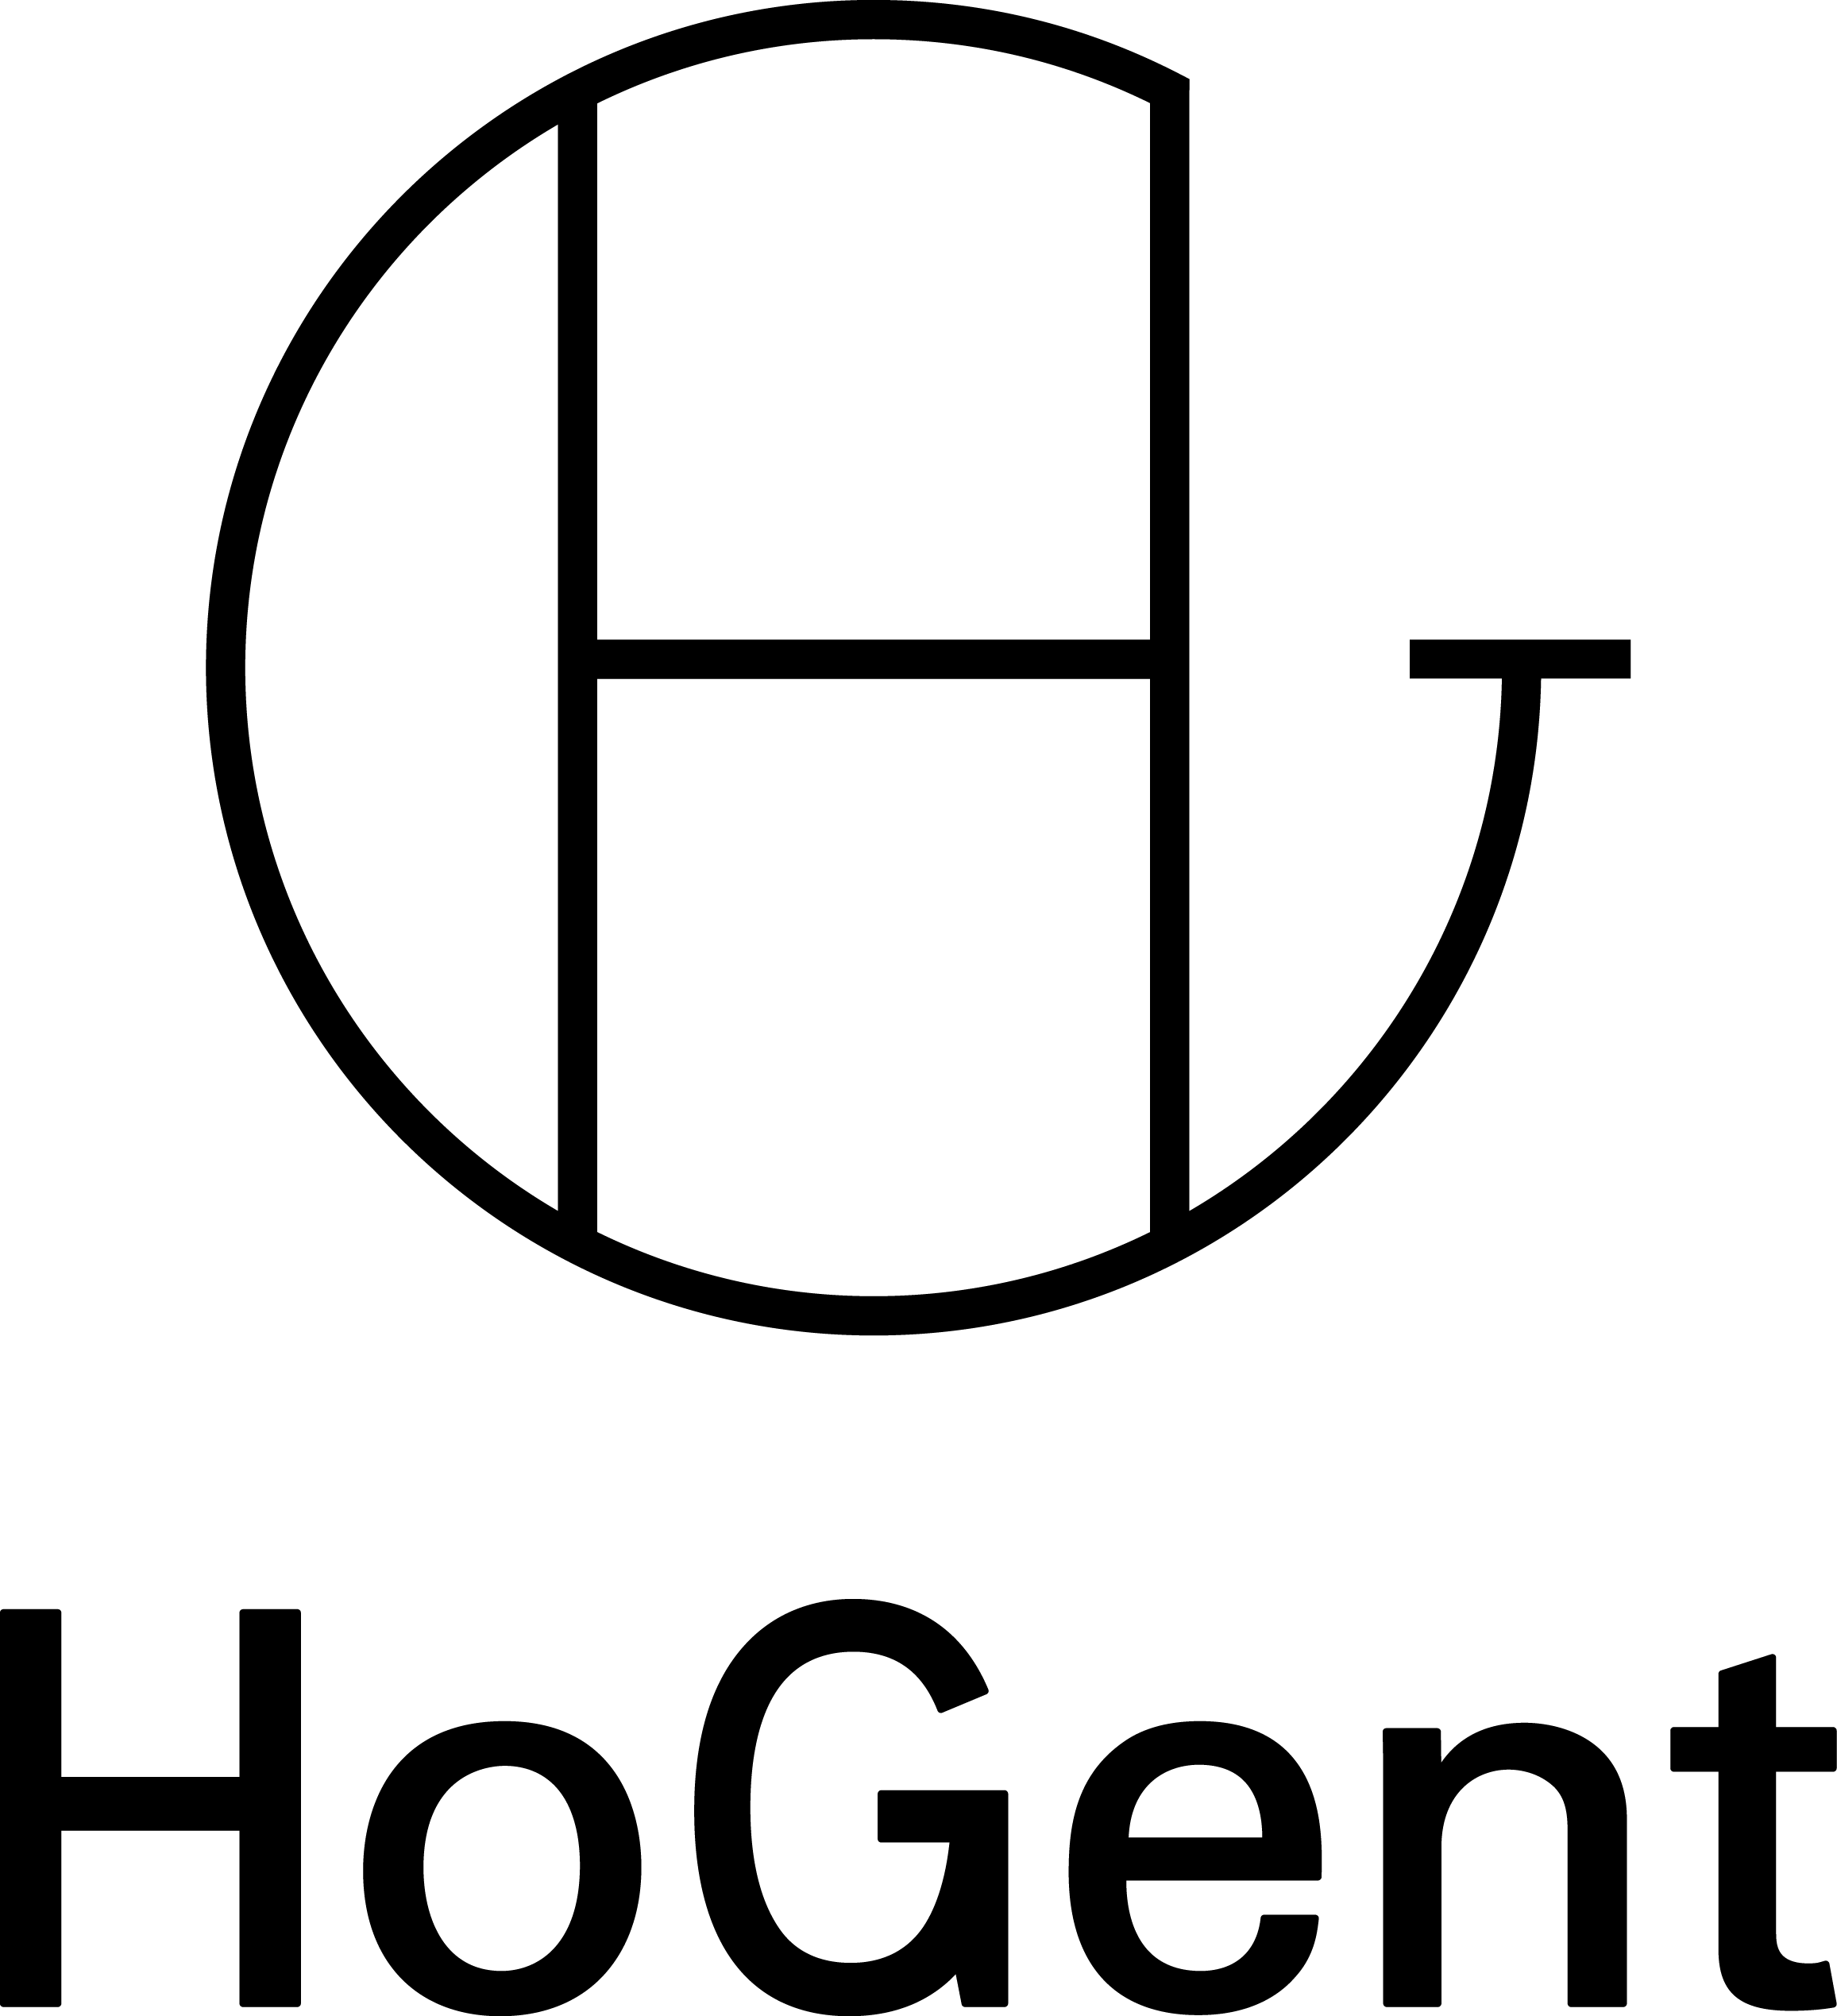
\includegraphics[width=2.5cm]{img/HG-beeldmerk-woordmerk}\\[.5cm]
    Faculteit Bedrijf en Organisatie\\[3cm]
    \titel
    \vfill
    \student\\[3.5cm]
    Scriptie voorgedragen tot het bekomen van de graad van\\professionele bachelor in de toegepaste informatica\\[2cm]
    Promotor:\\
    \promotor\\
    \ifdefempty{\copromotor}{\vspace{2.5cm}}{Co-promotor:\\\copromotor\\[2.5cm]}
    Instelling: \instelling\\[.5cm]
    Academiejaar: \academiejaar\\[.5cm]
    \ifcase \examenperiode \or Eerste \or Tweede \else Derde \fi examenperiode
    \endgroup

  \end{center}
  \restoregeometry
\end{titlepage}
  \emptypage
\begin{titlepage}
  \newgeometry{top=5.35cm,bottom=1.5cm,left=1.5cm,right=1.5cm}
  \begin{center}

    \begingroup
    \rmfamily
    \IfLanguageName{dutch}{Faculteit Bedrijf en Organisatie}{Faculty of Business and Information Management}\\[3cm]
    \titel
    \vfill
    \student\\[3.5cm]
    \IfLanguageName{dutch}{Scriptie voorgedragen tot het bekomen van de graad van\\professionele bachelor in de toegepaste informatica}{Thesis submitted in partial fulfillment of the requirements for the degree of\\professional bachelor of applied computer science}\\[2cm]
    Promotor:\\
    \promotor\\
    \ifdefempty{\copromotor}{\vspace{2.5cm}}{Co-promotor:\\\copromotor\\[2.5cm]}
    \IfLanguageName{dutch}{Instelling}{Institution}: \instelling\\[.5cm]
    \IfLanguageName{dutch}{Academiejaar}{Academic year}: \academiejaar\\[.5cm]
    \IfLanguageName{dutch}{%
    \ifcase \examenperiode \or Eerste \or Tweede \else Derde \fi examenperiode}{%
    \ifcase \examenperiode \or First \or Second \else Third \fi examination period}
    \endgroup

  \end{center}
  \restoregeometry
\end{titlepage}
}

%----------------------------------------------------------------------------------------
%	BIBLIOGRAPHY AND INDEX
%----------------------------------------------------------------------------------------

\usepackage[style=apa,backend=biber]{biblatex}
\usepackage{csquotes}
\DeclareLanguageMapping{dutch}{dutch-apa}
\addbibresource{bachproef-tin.bib} % BibTeX bibliography file
\defbibheading{bibempty}{}

\usepackage{calc} % For simpler calculation - used for spacing the index letter headings correctly
\usepackage{makeidx} % Required to make an index
\makeindex % Tells LaTeX to create the files required for indexing

%----------------------------------------------------------------------------------------
%	MAIN TABLE OF CONTENTS
%----------------------------------------------------------------------------------------

\usepackage{titletoc} % Required for manipulating the table of contents

\contentsmargin{0cm} % Removes the default margin

% Part text styling
\titlecontents{part}[0cm]
{\addvspace{20pt}\centering\large\bfseries}
{}
{}
{}

% Chapter text styling
\titlecontents{chapter}[1.25cm] % Indentation
{\addvspace{12pt}\large\sffamily\bfseries} % Spacing and font options for chapters
{\color{maincolor!60}\contentslabel[\Large\thecontentslabel]{1.25cm}\color{maincolor}} % Chapter number
{\color{maincolor}}
{\color{maincolor!60}\normalsize\;\titlerule*[.5pc]{.}\;\thecontentspage} % Page number

% Section text styling
\titlecontents{section}[1.25cm] % Indentation
{\addvspace{3pt}\sffamily\bfseries} % Spacing and font options for sections
{\contentslabel[\thecontentslabel]{1.25cm}} % Section number
{}
{\hfill\color{black}\thecontentspage} % Page number
[]

% Subsection text styling
\titlecontents{subsection}[1.25cm] % Indentation
{\addvspace{1pt}\sffamily\small} % Spacing and font options for subsections
{\contentslabel[\thecontentslabel]{1.25cm}} % Subsection number
{}
{\ \titlerule*[.5pc]{.}\;\thecontentspage} % Page number
[]

% List of figures
\titlecontents{figure}[0em]
{\addvspace{-5pt}\sffamily}
{\thecontentslabel\hspace*{1em}}
{}
{\ \titlerule*[.5pc]{.}\;\thecontentspage}
[]

% List of tables
\titlecontents{table}[0em]
{\addvspace{-5pt}\sffamily}
{\thecontentslabel\hspace*{1em}}
{}
{\ \titlerule*[.5pc]{.}\;\thecontentspage}
[]

%----------------------------------------------------------------------------------------
%	MINI TABLE OF CONTENTS IN PART HEADS
%----------------------------------------------------------------------------------------

% Chapter text styling
\titlecontents{lchapter}[0em] % Indenting
{\addvspace{15pt}\large\sffamily\bfseries} % Spacing and font options for chapters
{\color{maincolor}\contentslabel[\Large\thecontentslabel]{1.25cm}\color{maincolor}} % Chapter number
{}
{\color{maincolor}\normalsize\sffamily\bfseries\;\titlerule*[.5pc]{.}\;\thecontentspage} % Page number

% Section text styling
\titlecontents{lsection}[0em] % Indenting
{\sffamily\small} % Spacing and font options for sections
{\contentslabel[\thecontentslabel]{1.25cm}} % Section number
{}
{}

% Subsection text styling
\titlecontents{lsubsection}[.5em] % Indentation
{\normalfont\footnotesize\sffamily} % Font settings
{}
{}
{}

%----------------------------------------------------------------------------------------
%	PAGE HEADERS
%----------------------------------------------------------------------------------------

\usepackage{fancyhdr} % Required for header and footer configuration

\pagestyle{fancy}
\renewcommand{\chaptermark}[1]{\markboth{\sffamily\normalsize\bfseries\chaptername\ \thechapter.\ #1}{}} % Chapter text font settings
\renewcommand{\sectionmark}[1]{\markright{\sffamily\normalsize\thesection\hspace{5pt}#1}{}} % Section text font settings
\fancyhf{} \fancyhead[LE,RO]{\sffamily\normalsize\thepage} % Font setting for the page number in the header
\fancyhead[LO]{\rightmark} % Print the nearest section name on the left side of odd pages
\fancyhead[RE]{\leftmark} % Print the current chapter name on the right side of even pages
\renewcommand{\headrulewidth}{0.5pt} % Width of the rule under the header
\addtolength{\headheight}{2.5pt} % Increase the spacing around the header slightly
\renewcommand{\footrulewidth}{0pt} % Removes the rule in the footer
\fancypagestyle{plain}{\fancyhead{}\renewcommand{\headrulewidth}{0pt}} % Style for when a plain pagestyle is specified

% Removes the header from odd empty pages at the end of chapters
\makeatletter
\renewcommand{\cleardoublepage}{
\clearpage\ifodd\c@page\else
\hbox{}
\vspace*{\fill}
\thispagestyle{empty}
\newpage
\fi}

%----------------------------------------------------------------------------------------
%	THEOREM STYLES
%----------------------------------------------------------------------------------------

\usepackage{amsmath,amsfonts,amssymb,amsthm} % For math equations, theorems, symbols, etc

\newcommand{\intoo}[2]{\mathopen{]}#1\,;#2\mathclose{[}}
\newcommand{\ud}{\mathop{\mathrm{{}d}}\mathopen{}}
\newcommand{\intff}[2]{\mathopen{[}#1\,;#2\mathclose{]}}
\newtheorem{notation}{Notation}[chapter]

% Boxed/framed environments
\newtheoremstyle{maincolornumbox}% % Theorem style name
{0pt}% Space above
{0pt}% Space below
{\normalfont}% % Body font
{}% Indent amount
{\small\bf\sffamily\color{maincolor}}% % Theorem head font
{\;}% Punctuation after theorem head
{0.25em}% Space after theorem head
{\small\sffamily\color{maincolor}\thmname{#1}\nobreakspace\thmnumber{\@ifnotempty{#1}{}\@upn{#2}}% Theorem text (e.g. Theorem 2.1)
\thmnote{\nobreakspace\the\thm@notefont\sffamily\bfseries\color{black}---\nobreakspace#3.}} % Optional theorem note
\renewcommand{\qedsymbol}{$\blacksquare$}% Optional qed square

\newtheoremstyle{blacknumex}% Theorem style name
{5pt}% Space above
{5pt}% Space below
{\normalfont}% Body font
{} % Indent amount
{\small\bf\sffamily}% Theorem head font
{\;}% Punctuation after theorem head
{0.25em}% Space after theorem head
{\small\sffamily{\tiny\ensuremath{\blacksquare}}\nobreakspace\thmname{#1}\nobreakspace\thmnumber{\@ifnotempty{#1}{}\@upn{#2}}% Theorem text (e.g. Theorem 2.1)
\thmnote{\nobreakspace\the\thm@notefont\sffamily\bfseries---\nobreakspace#3.}}% Optional theorem note

\newtheoremstyle{blacknumbox} % Theorem style name
{0pt}% Space above
{0pt}% Space below
{\normalfont}% Body font
{}% Indent amount
{\small\bf\sffamily}% Theorem head font
{\;}% Punctuation after theorem head
{0.25em}% Space after theorem head
{\small\sffamily\thmname{#1}\nobreakspace\thmnumber{\@ifnotempty{#1}{}\@upn{#2}}% Theorem text (e.g. Theorem 2.1)
\thmnote{\nobreakspace\the\thm@notefont\sffamily\bfseries---\nobreakspace#3.}}% Optional theorem note

% Non-boxed/non-framed environments
\newtheoremstyle{maincolornum}% % Theorem style name
{5pt}% Space above
{5pt}% Space below
{\normalfont}% % Body font
{}% Indent amount
{\small\bf\sffamily\color{maincolor}}% % Theorem head font
{\;}% Punctuation after theorem head
{0.25em}% Space after theorem head
{\small\sffamily\color{maincolor}\thmname{#1}\nobreakspace\thmnumber{\@ifnotempty{#1}{}\@upn{#2}}% Theorem text (e.g. Theorem 2.1)
\thmnote{\nobreakspace\the\thm@notefont\sffamily\bfseries\color{black}---\nobreakspace#3.}} % Optional theorem note
\renewcommand{\qedsymbol}{$\blacksquare$}% Optional qed square
\makeatother

% Defines the theorem text style for each type of theorem to one of the three styles above
\newcounter{dummy}
\numberwithin{dummy}{section}
\theoremstyle{maincolornumbox}
\newtheorem{theoremeT}[dummy]{Theorem}
\newtheorem{problem}{Problem}[chapter]
\newtheorem{exerciseT}{Exercise}[chapter]
\theoremstyle{blacknumex}
\newtheorem{exampleT}{Example}[chapter]
\theoremstyle{blacknumbox}
\newtheorem{vocabulary}{Vocabulary}[chapter]
\newtheorem{definitionT}{Definition}[section]
\newtheorem{corollaryT}[dummy]{Corollary}
\theoremstyle{maincolornum}
\newtheorem{proposition}[dummy]{Proposition}

%----------------------------------------------------------------------------------------
%	DEFINITION OF COLORED BOXES
%----------------------------------------------------------------------------------------

\lstset{
	breaklines=true,
    backgroundcolor=\color{black},
    basicstyle=\fontfamily{pcr}\selectfont\footnotesize\color{white},
    numbersep=5pt,
    language=bash
}

\RequirePackage[framemethod=default]{mdframed} % Required for creating the theorem, definition, exercise and corollary boxes

% Theorem box
\newmdenv[skipabove=7pt,
skipbelow=7pt,
backgroundcolor=black!5,
linecolor=maincolor,
innerleftmargin=5pt,
innerrightmargin=5pt,
innertopmargin=5pt,
leftmargin=0cm,
rightmargin=0cm,
innerbottommargin=5pt]{tBox}

% Exercise box
\newmdenv[skipabove=7pt,
skipbelow=7pt,
rightline=false,
leftline=true,
topline=false,
bottomline=false,
backgroundcolor=maincolor!10,
linecolor=maincolor,
innerleftmargin=5pt,
innerrightmargin=5pt,
innertopmargin=5pt,
innerbottommargin=5pt,
leftmargin=0cm,
rightmargin=0cm,
linewidth=4pt]{eBox}

% Definition box
\newmdenv[skipabove=7pt,
skipbelow=7pt,
rightline=false,
leftline=true,
topline=false,
bottomline=false,
linecolor=maincolor,
innerleftmargin=5pt,
innerrightmargin=5pt,
innertopmargin=0pt,
leftmargin=0cm,
rightmargin=0cm,
linewidth=4pt,
innerbottommargin=0pt]{dBox}

% Corollary box
\newmdenv[skipabove=7pt,
skipbelow=7pt,
rightline=false,
leftline=true,
topline=false,
bottomline=false,
linecolor=gray,
backgroundcolor=black!5,
innerleftmargin=5pt,
innerrightmargin=5pt,
innertopmargin=5pt,
leftmargin=0cm,
rightmargin=0cm,
linewidth=4pt,
innerbottommargin=5pt]{cBox}

% Creates an environment for each type of theorem and assigns it a theorem text style from the "Theorem Styles" section above and a colored box from above
\newenvironment{theorem}{\begin{tBox}\begin{theoremeT}}{\end{theoremeT}\end{tBox}}
\newenvironment{exercise}{\begin{eBox}\begin{exerciseT}}{\hfill{\color{maincolor}\tiny\ensuremath{\blacksquare}}\end{exerciseT}\end{eBox}}
\newenvironment{definition}{\begin{dBox}\begin{definitionT}}{\end{definitionT}\end{dBox}}
\newenvironment{example}{\begin{exampleT}}{\hfill{\tiny\ensuremath{\blacksquare}}\end{exampleT}}
\newenvironment{corollary}{\begin{cBox}\begin{corollaryT}}{\end{corollaryT}\end{cBox}}

%----------------------------------------------------------------------------------------
%	REMARK ENVIRONMENT
%----------------------------------------------------------------------------------------

\newenvironment{remark}{\par\vspace{10pt}\small % Vertical white space above the remark and smaller font size
\begin{list}{}{
\leftmargin=35pt % Indentation on the left
\rightmargin=25pt}\item\ignorespaces % Indentation on the right
\makebox[-2.5pt]{\begin{tikzpicture}[overlay]
\node[draw=maincolor!60,line width=1pt,circle,fill=maincolor!25,font=\sffamily\bfseries,inner sep=2pt,outer sep=0pt] at (-15pt,0pt){\textcolor{maincolor}{R}};\end{tikzpicture}} % Orange R in a circle
\advance\baselineskip -1pt}{\end{list}\vskip5pt} % Tighter line spacing and white space after remark

%----------------------------------------------------------------------------------------
%	SECTION NUMBERING IN THE MARGIN
%----------------------------------------------------------------------------------------

\makeatletter
\renewcommand{\@seccntformat}[1]{\llap{\textcolor{maincolor}{\csname the#1\endcsname}\hspace{1em}}}
\renewcommand{\section}{\@startsection{section}{1}{\z@}
{-4ex \@plus -1ex \@minus -.4ex}
{1ex \@plus.2ex }
{\normalfont\large\sffamily\bfseries}}
\renewcommand{\subsection}{\@startsection {subsection}{2}{\z@}
{-3ex \@plus -0.1ex \@minus -.4ex}
{0.5ex \@plus.2ex }
{\normalfont\sffamily\bfseries}}
\renewcommand{\subsubsection}{\@startsection {subsubsection}{3}{\z@}
{-2ex \@plus -0.1ex \@minus -.2ex}
{.2ex \@plus.2ex }
{\normalfont\small\sffamily\bfseries}}
\renewcommand\paragraph{\@startsection{paragraph}{4}{\z@}
{-2ex \@plus-.2ex \@minus .2ex}
{.1ex}
{\normalfont\small\sffamily\bfseries}}

%----------------------------------------------------------------------------------------
%	PART HEADINGS
%----------------------------------------------------------------------------------------

% numbered part in the table of contents
\newcommand{\@mypartnumtocformat}[2]{%
\setlength\fboxsep{0pt}%
\noindent\colorbox{maincolor!20}{\strut\parbox[c][.7cm]{\ecart}{\color{maincolor!70}\Large\sffamily\bfseries\centering#1}}\hskip\esp\colorbox{maincolor!40}{\strut\parbox[c][.7cm]{\linewidth-\ecart-\esp}{\Large\sffamily\centering#2}}}%
%%%%%%%%%%%%%%%%%%%%%%%%%%%%%%%%%%
% unnumbered part in the table of contents
\newcommand{\@myparttocformat}[1]{%
\setlength\fboxsep{0pt}%
\noindent\colorbox{maincolor!40}{\strut\parbox[c][.7cm]{\linewidth}{\Large\sffamily\centering#1}}}%
%%%%%%%%%%%%%%%%%%%%%%%%%%%%%%%%%%
\newlength\esp
\setlength\esp{4pt}
\newlength\ecart
\setlength\ecart{1.2cm-\esp}
\newcommand{\thepartimage}{}%
\newcommand{\partimage}[1]{\renewcommand{\thepartimage}{#1}}%
\def\@part[#1]#2{%
\ifnum \c@secnumdepth >-2\relax%
\refstepcounter{part}%
\addcontentsline{toc}{part}{\texorpdfstring{\protect\@mypartnumtocformat{\thepart}{#1}}{\partname~\thepart\ ---\ #1}}
\else%
\addcontentsline{toc}{part}{\texorpdfstring{\protect\@myparttocformat{#1}}{#1}}%
\fi%
\startcontents%
\markboth{}{}%
{\thispagestyle{empty}%
\begin{tikzpicture}[remember picture,overlay]%
\node at (current page.north west){\begin{tikzpicture}[remember picture,overlay]%
\fill[maincolor!20](0cm,0cm) rectangle (\paperwidth,-\paperheight);
\node[anchor=north] at (4cm,-3.25cm){\color{maincolor!40}\fontsize{220}{100}\sffamily\bfseries\@Roman\c@part};
\node[anchor=south east] at (\paperwidth-1cm,-\paperheight+1cm){\parbox[t][][t]{8.5cm}{
\printcontents{l}{0}{\setcounter{tocdepth}{1}}%
}};
\node[anchor=north east] at (\paperwidth-1.5cm,-3.25cm){\parbox[t][][t]{15cm}{\strut\raggedleft\color{white}\fontsize{30}{30}\sffamily\bfseries#2}};
\end{tikzpicture}};
\end{tikzpicture}}%
\@endpart}
\def\@spart#1{%
\startcontents%
\phantomsection
{\thispagestyle{empty}%
\begin{tikzpicture}[remember picture,overlay]%
\node at (current page.north west){\begin{tikzpicture}[remember picture,overlay]%
\fill[maincolor!20](0cm,0cm) rectangle (\paperwidth,-\paperheight);
\node[anchor=north east] at (\paperwidth-1.5cm,-3.25cm){\parbox[t][][t]{15cm}{\strut\raggedleft\color{white}\fontsize{30}{30}\sffamily\bfseries#1}};
\end{tikzpicture}};
\end{tikzpicture}}
\addcontentsline{toc}{part}{\texorpdfstring{%
\setlength\fboxsep{0pt}%
\noindent\protect\colorbox{maincolor!40}{\strut\protect\parbox[c][.7cm]{\linewidth}{\Large\sffamily\protect\centering #1\quad\mbox{}}}}{#1}}%
\@endpart}
\def\@endpart{\vfil\newpage
\if@twoside
\if@openright
\null
\thispagestyle{empty}%
\newpage
\fi
\fi
\if@tempswa
\twocolumn
\fi}

%----------------------------------------------------------------------------------------
%	CHAPTER HEADINGS
%----------------------------------------------------------------------------------------

% A switch to conditionally include a picture, implemented by  Christian Hupfer
\newif\ifusechapterimage
\usechapterimagetrue
\newcommand{\thechapterimage}{}%
\newcommand{\chapterimage}[1]{\ifusechapterimage\renewcommand{\thechapterimage}{#1}\fi}%
\def\@makechapterhead#1{%
{\parindent \z@ \raggedright \normalfont
\ifnum \c@secnumdepth >\m@ne
\if@mainmatter
\begin{tikzpicture}[remember picture,overlay]
\node at (current page.north west)
{\begin{tikzpicture}[remember picture,overlay]
\node[anchor=north west,inner sep=0pt] at (0,0) {\ifusechapterimage\includegraphics[width=\paperwidth]{\thechapterimage}\fi};
\draw[anchor=west] (\Gm@lmargin,-9cm) node [line width=2pt,rounded corners=15pt,draw=maincolor,fill=white,fill opacity=0.5,inner sep=15pt]{\strut\makebox[22cm]{}};
\draw[anchor=west] (\Gm@lmargin+.3cm,-9cm) node {\huge\sffamily\bfseries\color{black}\thechapter. #1\strut};
\end{tikzpicture}};
\end{tikzpicture}
\else
\begin{tikzpicture}[remember picture,overlay]
\node at (current page.north west)
{\begin{tikzpicture}[remember picture,overlay]
\node[anchor=north west,inner sep=0pt] at (0,0) {\ifusechapterimage\includegraphics[width=\paperwidth]{\thechapterimage}\fi};
\draw[anchor=west] (\Gm@lmargin,-9cm) node [line width=2pt,rounded corners=15pt,draw=maincolor,fill=white,fill opacity=0.5,inner sep=15pt]{\strut\makebox[22cm]{}};
\draw[anchor=west] (\Gm@lmargin+.3cm,-9cm) node {\huge\sffamily\bfseries\color{black}#1\strut};
\end{tikzpicture}};
\end{tikzpicture}
\fi\fi\par\vspace*{270\p@}}}

%-------------------------------------------

\def\@makeschapterhead#1{%
\begin{tikzpicture}[remember picture,overlay]
\node at (current page.north west)
{\begin{tikzpicture}[remember picture,overlay]
\node[anchor=north west,inner sep=0pt] at (0,0) {\ifusechapterimage\includegraphics[width=\paperwidth]{\thechapterimage}\fi};
\draw[anchor=west] (\Gm@lmargin,-9cm) node [line width=2pt,rounded corners=15pt,draw=maincolor,fill=white,fill opacity=0.5,inner sep=15pt]{\strut\makebox[22cm]{}};
\draw[anchor=west] (\Gm@lmargin+.3cm,-9cm) node {\huge\sffamily\bfseries\color{black}#1\strut};
\end{tikzpicture}};
\end{tikzpicture}
\par\vspace*{270\p@}}
\makeatother

%----------------------------------------------------------------------------------------
%	HYPERLINKS IN THE DOCUMENTS
%----------------------------------------------------------------------------------------

\usepackage{hyperref}
\hypersetup{hidelinks,backref=true,pagebackref=true,hyperindex=true,colorlinks=false,breaklinks=true,urlcolor= maincolor,bookmarks=true,bookmarksopen=false,pdftitle={Title},pdfauthor={Author}}
\usepackage{bookmark}
\bookmarksetup{
open,
numbered,
addtohook={%
\ifnum\bookmarkget{level}=0 % chapter
\bookmarksetup{bold}%
\fi
\ifnum\bookmarkget{level}=-1 % part
\bookmarksetup{color=maincolor,bold}%
\fi
}
}

%----------------------------------------------------------------------------------------
%	Java source code
%----------------------------------------------------------------------------------------

% Commando voor invoegen Java-broncodebestanden (dank aan Niels Corneille)
% Gebruik:
%   \codefragment{source/MijnKlasse.java}{Uitleg bij de code}
%
% Je kan dit aanpassen aan de taal die je zelf het meeste gebruikt in je
% bachelorproef.
\newcommand{\codefragment}[2]{ \lstset{%
  language=java,
  breaklines=true,
  float=th,
  caption={#2},
  basicstyle=\scriptsize,
  frame=single,
  extendedchars=\true
}
\lstinputlisting{#1}}

% Leeg blad
\newcommand{\emptypage}{%
\newpage
\thispagestyle{empty}
\mbox{}
\newpage
}


%%---------- Documenteigenschappen --------------------------------------------
%% TODO: Vul dit aan met je eigen info:

% Je eigen naam
\newcommand{\student}{Mike Heymans}

% De naam van je promotor (lector van de opleiding)
\newcommand{\promotor}{Koen Hoof}

% De naam van je co-promotor. Als je promotor ook je opdrachtgever is en je
% dus ook inhoudelijk begeleidt (en enkel dan!), mag je dit leeg laten.
\newcommand{\copromotor}{Steven Rymenans}

% Indien je bachelorproef in opdracht van/in samenwerking met een bedrijf of
% externe organisatie geschreven is, geef je hier de naam. Zoniet laat je dit
% zoals het is.
\newcommand{\instelling}{---}

% De titel van het rapport/bachelorproef
\newcommand{\titel}{Adobe Experience Manager: omgaan met dynamische data}

% Datum van indienen (gebruik telkens de deadline, ook al geef je eerder af)
\newcommand{\datum}{2 juni 2017}

% Academiejaar
\newcommand{\academiejaar}{2016-2017}

% Examenperiode
%  - 1e semester = 1e examenperiode => 1
%  - 2e semester = 2e examenperiode => 2
%  - tweede zit  = 3e examenperiode => 3
\newcommand{\examenperiode}{2}

%%=============================================================================
%% Inhoud document
%%=============================================================================

\begin{document}

%---------- Taalselectie ------------------------------------------------------
%% Als je je bachelorproef in het Engels schrijft, haal dan onderstaande regel
%% uit commentaar. Let op: de tekst op de voorkaft blijft in het Nederlands, en
%% dat is ook de bedoeling!
%\selectlanguage{english}

%---------- Titelblad ---------------------------------------------------------
\inserttitlepage
\usechapterimagefalse

%---------- Samenvatting, voorwoord -------------------------------------------

	% !TeX spellcheck = nl_NL
\documentclass{article}

\begin{document}
	\section{Samenvatting}
Adobe Experience Manager operationeel krijgen is niet vanzelfsprekend, er komen verschillende frameworks aan bod die elk een studie op zich kunnen vormen. Eenmaal opgezet blijft de vraag van hoe we met de dynamische data moeten omgaan en wat de vuistregels zijn. Omdat de Adobe documentatie beperkt geeft deze scriptie een beschrijf van de opzet en omgang van AEM.
\par
Om te begrijpen wat de verschillende lagen zijn van AEM en hoe deze met elkaar communiceren bouwen we een volledige stack die gebruikt kan worden om mee te experimenteren. Deze stack bestaat uit een webapplicatie opgezet met AEM, een simplistische webcatalogus waar gebruikers aan de hand van categori\"een producten kunnen opzoeken. We voorzien tevens een databank die dienst zal doen als ERP, records in de databank wijzigen en moeten op onze website doorkomen. Bij het bouwen van deze stack gaan we op zoek naar manier om dit te realiseren.
\par
Bij het onderzoek hebben we vier methoden onderzocht om met onze dynamische data om te gaan. De eerste zijnde pagina's laten genereren op basis van data uit de databank. Dit is een dure operatie en kan voor problemen zorgen bij onbezonnen gebruik maar is de enigste manier om editeerbare pagina's aan de hand van dynamische pagina te voorzien. De tweede manier is de data ophalen wanneer deze nodig is om vervolgens een pagina aan te maken. Deze methode is toepasbaar op een grote dataset maar ontbreekt aan de mogelijkheid om de pagina te editeren. Vervolgens hebben we Server Side Includes als optie beschouwt, hiermee kan men verschillende datatypes injecteren in een reeds bestaande html. Het voordeel hierbij is de mogelijkheid om de html apart van de data te cachen waardoor deze optie een performantie-boost ondervindt. Het nadeel van SSI is dat deze server side werkt waardoor het onmogelijk is om hiermee een interactieve pagina op te bouwen. Hiervoor hebben we onze vierde methode nodig, JavaScript. JavaScript is de enige manier om een interactieve UI te voorzien zonder pagina's opnieuw te hoeven inladen na een actie van de gebruiker.
\par
We kunnen besluiten dat AEM opties heeft voor dynamische data maar dat het belangrijk is om voor de ontwikkeling aanvangt een duidelijk overzicht te krijgen van de veranderlijkheid ervan en in welke situaties de gebruiker deze nodig zal hebben. Het is van het grootste belang dat een nieuwe applicatie zorgvuldig wordt gedissecteerd en de data gecatalogiseerd zodat weet welke methode waar toe te passen. Dit zorgt voor een functionele applicatie met oog op performantie alsook een kortere ontwikkelingstijd.
\end{document}
	% !TeX spellcheck = nl_NL
\documentclass{article}

\begin{document}
	\section{Voorwoord}
	In het kader van mijn opleiding Toegepaste Informatica aan de Hogeschool Gent
	heb ik onderzoek gedaan naar het Adobe Experience Manager platform, beter gekend als AEM. 
	Het resultaat dat nu voor u ligt is er \'e\'en van drie maanden hard werk waarin heel wat gevloek heeft plaatsgevonden. 
	In nazicht van dit onderzoek ben ik tevreden over het resultaat maar vooral voldaan met de verworven kennis. 
	Al heeft deze kennis gezorgd voor nieuwe vraagtekens die in de toekomst mijn aandacht zullen opslorpen.
	\par
	\par
	Deze proef was niet mogelijk geweest zonder de inzet van AS Adventure, die zo vriendelijk waren om een licentie
	beschikbaar te stellen alsook mij te begeleiden in mijn ontdekkingsreis binnen de wereld van AEM. 
	Ik wil ook mijn collega’s bedanken voor hun uitmuntende begeleiding en eindeloos geduld.
	\par
	In het bijzonder wil ik mijn begeleiders Koen Hoof en Steven Rymenans bedanken voor hun ondersteuning tijdens deze reis.
	\par
	Veel plezier met het lezen van deze scriptie.
\end{document}
	

%---------- Inhoudstafel ------------------------------------------------------
\pagestyle{empty} % No headers
\tableofcontents % Print the table of contents itself
\cleardoublepage % Forces the first chapter to start on an odd page so it's on the right
\pagestyle{fancy} % Print headers again

	
%---------- Lijst afkortingen, termen -----------------------------------------
%% Als je een lijst van afkortingen of termen wil toevoegen, dan hoort die
%% hier thuis. Gebruik bijvoorbeeld de ``glossaries'' package.

%%---------- Kern -------------------------------------------------------------

	\chapter{Inleiding}
	% !TeX spellcheck = nl_NL
\documentclass{article}

\begin{document}
	\section{Reden van onderzoek}
	Adobe Experience Manager is het gelicentieerde  contentmanagementsysteem (CMS) van Adobe. 
	Een CMS-applicatie maakt het mogelijk voor mensen zonder kennis van HTML of CSS om webpagina’s aan te maken of te wijzigen. 
	Het is ideaal voor websites die vaak de inhoud van hun site wijzigen of snel willen inspelen op actuele gebeurtenissen. 
	Dit komt doordat designers en marketeers zelf de pagina's kunnen editeren in plaats van eerst content uit te denken en de realisatie over te laten aan een front-end developer. 
	\par
	Toen AS Adventure besloot om zijn huidige website, en die van zijn zusterbedrijven, niet langer uit te besteden aan een extern bedrijf maar deze intern te gaan beheren en ontwikkelen, is er besloten om deze met het AEM-platform op te zetten. 
	Dit zou het bedrijf in staat stellen zijn content volledig door de designers te laten beheren, zonder tussenkomst van developers.
	Denk maar aan de homepage die van achtergrondafbeelding wijzigt of een gepersonaliseerde pagina voor een merk, allemaal mogelijk dankzij AEM.
	\par
	Dat dit allemaal out-of-the-box mogelijk is, is te mooi om waar te zijn. Voor het content team aan de slag kan, moeten er componenten gebouwd worden, dit is het werk van de ontwikkelaars. Eigenlijk komt het erop neer dat componenten de bakstenen vormen om een website op te bouwen en de designers zijn de metsers. Ze kunnen lustig huisjes bouwen, maar wanneer er nood is aan een baksteen met een nieuwe feature moet hiervoor een aanvraag gedaan worden bij de steenbakkers, gespeeld door de ontwikkelaars. Deze stenen bevatten niet enkel HTML en CSS maar ook Java (en diverse frameworks) zijn nodig om dit nieuw type steen te ontwikkelen. De designers krijgen de nieuwe baksteen en kunnen hiermee aan de slag gaan.
	\par
	Buiten de content die door het marketingteam wordt voorzien is er ook data die vanuit een databank moet komen. 
	Hierbij hebben we het over records die niet manueel worden aangepast maar met duizenden tegelijk of data die niet enkel betrekking hebben op de site maar ook tijdens andere processen een rol spelen. 
	Een voorbeeld hiervan zijn de prijzen, tijdens de solden is het niet re\"eel om elke prijs handmatig aan te passen op de pagina’s. 
	In het onwaarschijnlijke geval dat het handmatig aanpassen van een specifieke prijs nodig is, zou deze data enkel op de pagina gewijzigd zijn en niet in het ERP. 
	Het is dus logischer dat het ERP deze wijziging doet en door duwt naar de pagina. Ook hier spelen de ontwikkelaars een rol, het is hun taak de systemen die dit mogelijk maken te bedenken en te realiseren.
	\par
	Toen AS Adventure aan dit project begon waren er processen uitgedacht om deze wijzigingen weer te geven en toen de eerste twee sites, Juttu en Yaya, live stonden was iedereen tevreden over het resultaat. 
	Maar deze shops zijn relatief nieuw en beperkt in aanbod, toen de vernieuwde AS Adventure site live ging staken er enkele problemen de kop op. Aangezien deze problemen in productie voorkwamen was wachten geen optie en moesten deze opgelost worden, niet zozeer met de beste maar wel de snelste oplossing.
	\par
	Deze proef heeft als nut het herzien van wat er tot nu toe opgebouwd werd, hoe het AEM-platform aangepast is geweest om aan de behoeften te voldoen en of dit ook effectief de beste manier is om de vereiste functionaliteit te bekomen. 
    Door het in kaart brengen van onze methodologi\"en hopen we een dieper inzicht te verwerven in het platform alsook een leidraad te voorzien voor ontwikkelaars die een eerste keer kennis maken met AEM of zij die reeds werken met AEM en geconfronteerd worden met de problemen waarvoor wij een oplossing zoeken. 
	Zoals het gezegde luidt: het is goed te leren van je fouten maar beter om te leren uit die van een ander.
\end{document}
	
	\chapter{De REST service}
	% !TeX spellcheck = nl_NL
\documentclass{article}

\begin{document}
	\section{De database}
	Om onze AEM-applicatie te bouwen hebben we nood aan een database waaruit we onze informatie kunnen halen.
	De manier waarop we deze informatie halen zal afhangen van model tot model daarom zullen we elke mogelijkheid
	proberen te voorzien tijdens de opzet.

\end{document}
	% !TeX spellcheck = nl_NL
\documentclass{article}

\begin{document}
	\subsection{Apache Cassandra}
	Apache Cassandra is een open-source NoSql (Not only Sql) database die de dag van vandaag door vele internationale bedrijven 
	in gebruik is genomen. 
	Netflix, Instagram en het CERN hebben in Cassandra een performante, stabiele databank gevonden, 
	die de beschikbaarheid van hun data garandeert.
	\par
	\begin{wrapfigure}{l}{0.5\textwidth}
  		
\includegraphics[width=0.4\textwidth]{images/cassandra.png}
	\end{wrapfigure}
	Deze garantie wordt geboden door de structuur waarmee Cassandra data beheert. 
	Een databank bestaat uit een collectie van noden die een cluster vormen. 
	Het beheer gebeurt decentraal, elke node heeft dezelfde rol, 
	dit maakt dat wanneer een node offline is, de andere ongehinderd blijven werken. 
	Om het volle potentieel van Cassandra te benutten, is het aangeraden om de noden niet enkel over verschillende servers 
	maar ook over verschillende datacenters te verspreiden. 
	Bij deze setup mag er een datacenter offline gaan, de gebruiker zal hier geen weet van hebben.  
	En wanneer het datacenter terug online is, zal de data gedeeld worden met de herstelde noden.
	Dit is ook positief voor de schaalbaarheid. 
	Wanneer een node wordt toegevoegd, haalt deze zijn configuratie op bij een bestaande node en sluit zich naadloos aan in de cluster.
	\par
	Bij het aanmaken van een cluster kan men een replicatie factor meegeven. 
	Deze geeft aan op hoeveel verschillende noden een record moet bewaard worden. 
	Bij een factor 3 zal elk record op 3 noden beschikbaar zijn. 
	Des te groter de factor, des te groter de performantie en stabiliteit maar ook de duplicatie aan data vergroot mee.
	Bij het kiezen van de replicatiefactor moet er een afweging gemaakt worden tussen niveau van beschikbaarheid en
	de extra load veroorzaakt door het schrijven naar meerdere noden.
	\par
	Een groot verschil met een relationele databank is dat het linken van verscheidene tabellen niet mogelijk is.
	In plaats daarvan werkt Cassandra met collecties die rechtstreeks in een kolom worden opgeslagen. 
	Dit wordt mogelijk door het aanmaken van UDTs (User Defined Types). 
	Wanneer een lijst van UDTs (of primitieve types) wordt opgeslagen, wordt deze omgevormd naar een JSON-achtige structuur. 
	Doordat alle data in \'e\'en rij zitten, hoeven er geen joins gedaan te worden over meerdere tabellen 
	wat de performantie aanzienlijk verhoogt.
	\par
	Er zijn ook enkele nadelen verbonden aan het kiezen voor Cassandra als database, \'e\'en van deze nadelen is dat het, out-of-the-box,
	onmogelijk is om tabellen te queri\"en zoals je met een relationele databank zou doen. 
	Dit komt doordat Cassandra werkt met key-value paren om de data op te slagen en dus enkel aan de hand van een key 
	(of deel van een key) naar een record gezocht kan worden. 
	Een neveneffect hiervan is dat aggregatie functies enkel op partitie niveau kunnen worden uitgevoerd.
	\par
	Aangezien Cassandra een non-relationele databank is, is een ander nadeel de afwezigheid van transacties op databank niveau.
	Enkel op rijniveau kan men gebruik maken van lightweight transacties door een conditie toe te voegen voor een schrijf operatie.
	Hiervoor zou men een versie kunnen toevoegen aan een tabel zodat wanneer men een schrijf operatie wil doen,
	er gekeken kan worden of de versie nog overeenstemt. 
	Indien dit niet het geval is, wordt de operatie niet uitgevoerd en kan het systeem op een gepaste manier reageren.
\end{document}
	
	% !TeX spellcheck = nl_NL
\documentclass{article}

\begin{document}
	\subsection{Een Cassandra cluster opzetten}
	Nu we onze databank gekozen hebben, is het tijd dat we deze opzetten. 
	De stappen die nodig zijn, beginnend van niets, om een cluster op te zetten worden in dit segment besproken. 
	We zullen eerst de machines aanmaken, vervolgens Cassandra installeren en als laatste stap onze nodes met elkaar in contact brengen.
	Voor dit project heb ik gekozen om met 3 nodes te werken, dit om toch enige performantie te hebben zonder het prijzig te maken.
	\subsubsection{De machines}
	Als eerste maken we de 3 machines aan waarop we Cassandra zullen draaien. 
	Via de AWS-console navigeren we naar EC2 -> Instances waar we de ‘Launch instance’ kiezen.
	Het eerste scherm laat ons kiezen welk besturingssysteem we willen gebruiken, hier kiezen we Amazon Linux AMI. 
	In stap 2 bepalen we hoe krachtig onze machines zullen zijn. Het is perfect mogelijk om met de t2.micro 
	(deze is gratis te gebruiken bij een ‘Free Tier’) maar met slecht 1 CPU en 1GB RAM heeft deze niet zo veel te bieden. 
	Hier heb ik voor de t2.large geopteerd, deze zal beter aansluiten bij onze behoeften. 
	Stap 3 hoeven we enkel het aantal instances dat we willen aanmaken wijzigen naar 3, 
	de rest laten we ongewijzigd. Stap 4 en 5 slagen we over, deze zijn niet van toepassing. 
	In Stap 6 maken we een nieuwe security group aan die de poorten nodig voor het gebruik van onze databank openzet. 
	Voor onderstaande poorten maken we een ‘Custom TCP Rule’ en maken we ze compleet publiek (in productie omgevingen is 
	dit ten strengste af te raden.) door de toegestane IP-adressen op ‘0.0.0.0/0’ te zetten. 	Figuur \ref{fig:security-settings} toont ons hoe we dit bekomen.
	
	
	
	\begin{figure}[h!]
  		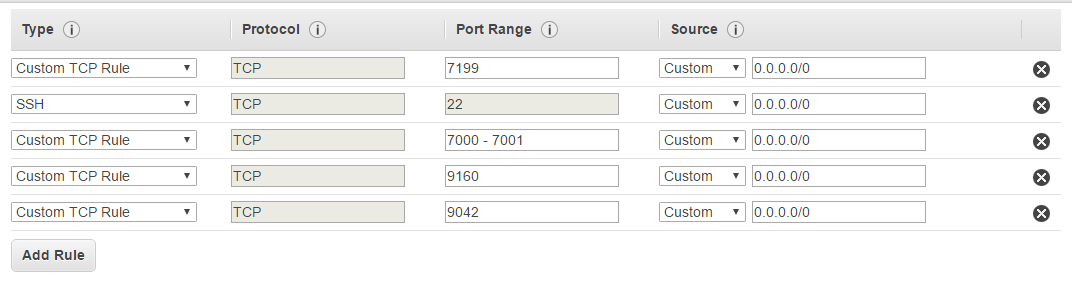
\includegraphics[width=\linewidth]{images/inbound-rules-cassandra.PNG}
  		\caption{security settings.}
  		\label{fig:security-settings}
	\end{figure}
	
	\par
	Indien deze stap afgehandeld is, krijgen we een overzicht te zien. 
	Als alles naar wens is klikken we op ‘Launch’ waardoor er een prompt opengaat. 
	Vanuit deze prompt kunnen we een pem-file aanmaken en downloaden, het is zeer belangrijk om 
	deze op een veilige plaats op te slaan, deze nodig is om via ssh een connectie naar onze machines te maken. 
	Bij het aanmaken van nieuwe machines kunnen we dezelfde pem-file hergebruiken zodat we één key hebben voor al onze instances.
	 We slagen het bestand op onder aem-ec2.pem.
	
	\subsubsection{Cassandra als service}
	Nu we onze machines hebben is het tijd om hiervan Cassandra nodes te maken. 
	Via het ‘Instance’ scherm kunnen we achterhalen wat de publieke IP-adressen zijn van deze machines 
	(laten we ervan uitgaan dat deze 1.0.0.1,1.0.0.2 en 1.0.0.3 zijn.). 
	Volgende stap moet op elke machine identiek herhaalt worden buiten de nodige aanpassingen aan de cassandra.yaml. 
	Laten we eerst op onze machines inloggen via het commando:
	
	\begin{lstlisting}
		$ ssh –i aem-ec2.pem ec2-user@1.0.0.1 
	\end{lstlisting}
	
	Nu zijn we ingelogd als ec2-user op onze machine. Om Cassandra 3.x te kunnen draaien hebben we Java 1.8 nodig, 
	via het commando ‘java -version’ kunnen we dit controleren. 
	Indien de versie lager ligt, zijn we verplicht om Java 1.8 te installeren. Een mogelijke manier om dit te doen is als volgt:	
	\par
	We navigeren naar onze jvm folder
	\begin{lstlisting}
  		$ cd /usr/lib/jvm
	\end{lstlisting}
	\par
	Vervolgens downloaden we de java 1.8 tar file
	\begin{lstlisting}
		$ sudo wget --no-cookies --no-check-certificate --header "Cookie: gpw_e24=http://www.oracle.com/; oraclelicense=accept-securebackup-cookie" http://download.oracle.com/otn-pub/java/jdk/8u121-b13/e9e7ea248e2c4826b92b3f075a80e441/jdk-8u121-linux-x64.tar.gz
	\end{lstlisting}
	
	\par
	En pakken we deze uit
	\begin{lstlisting}
		$ sudo tar xzf jdk-8u121-linux-x64.tar.gz
	\end{lstlisting}
	
	\par
	Na het uitpakken kunnen we onze jdk registreren als java optie
	\begin{lstlisting}
		$ sudo alternatives --install /usr/bin/java java /usr/lib/jvm/jdk1.8.0_121/bin/java 2
	\end{lstlisting}
	
	\par
	Als we nu het volgende commando runnen zien we twee java mogelijke java engines, diegene dat al geïnstalleerd was en onze nieuwe. 
	Hier kiezen we om onze nieuwe als default te gebruiken.
	\begin{lstlisting}
		$ sudo alternatives --config java
	\end{lstlisting}
	\begin{lstlisting}
		$ Enter to keep the current selection[+], or type selection number: 2
	\end{lstlisting}
	
	\par
	Als alles correct verlopen is zien we nu 1.8 staan wanneer we opnieuw het commando ‘java -version’ uitvoeren.
	
	\par
	Nu volgt de installatie van Cassandra zelf, hierbij is de eerste stap het toevoegen van de datastax.repo zodat we via het yum commando Cassandra kunnen installeren.
	 Als dit gebeurt is kunnen we via yum zowel Cassandra als Nodetool installeren.
	\par
	Maak het bestand datastax.repo aan.
	\begin{lstlisting}
		$ sudo touch /etc/yum.repos.d/datastax.repo
	\end{lstlisting}
	
	\par
	Maak het bestand datastax.repo aan.
	\begin{lstlisting}
		$ sudo touch /etc/yum.repos.d/datastax.repo
	\end{lstlisting}
	
	\par
	Vul deze met de nodige data
	\begin{lstlisting}
		$ sudo touch /etc/yum.repos.d/datastax.repo
	\end{lstlisting}
	En zorg dat deze conform is aan Figuur \ref{fig:datastax.repo}
	\begin{figure}[h!]
  		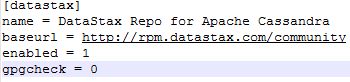
\includegraphics[width=\linewidth]{images/datastax-repo.PNG}
  		\caption{datastax.repo}
  		\label{fig:datastax.repo}
	\end{figure}
	
	\par
	Nu kunnen we Cassandra en Nodetool installeren.
	\begin{lstlisting}
		$ sudo yum install dsc30
	\end{lstlisting}
	\begin{lstlisting}
		$ sudo yum install cassandra30-tools
	\end{lstlisting}
	
	\par
	Als we nu Cassandra zouden opstarten op de 3 machines, hebben we 3 clusters met elks 1 node gemaakt. 
	Vanzelfsprekend is dit niet het gezochte resultaat en willen we 1 cluster met 3 nodes, om dit mogelijk te maken moeten we de aanpassingen maken, getoond in Figuur \ref{fig:cassandra.yaml} (locatie: /etc/cassandra/conf/cassandra.yaml).
	\begin{figure}[h!]
  		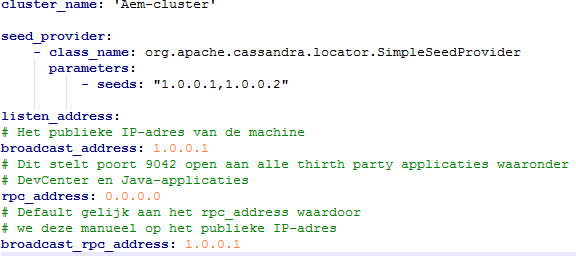
\includegraphics[width=\linewidth]{images/cassandra-yaml.PNG}
  		\caption{cassandra.yaml}
  		\label{fig:cassandra.yaml}
	\end{figure}
	
	\par
	Nu dat onze yamls correct staan kunnen we op onze machines cassandra starten met het commando ‘sudo service cassandra start’. 
	Na enkele minuten zien we dan dat de 3 nodes elkaar gevonden hebben via het commando ‘nodetool status’.
	
	\par
	\subsubsection{DevCenter}
	 Nu we onze databank hebben kunnen we onze nodige modellen toevoegen, het gebruikte script kan je terugvinden in de bijlagen.
	 Voor het uitvoeren van deze scripts kan gebruikt maken van DevCenter, een open-source tool waarmee een connectie kan gemaakt worden met een cluster. 
	 Deze manier van werken is aangenamer dan telkens te moeten sshen naar een node om daar via het cqlsh commando onze databank te kunnen querieën. 
	 Onze drie tabellen die we gaan gebruiken zijn Product, Category en Price. 
	 Deze drie vertonen elk een andere graad van dynamiek, gepast voor het onderzoek dat we zullen verrichten.
	 We voorzien telkens ook een log tabel voor deze drie zodat we aan de hand van een datum, die fungeert als ondergrends, de gewijzigde rijen kunnen opvragen.
	 Eenmaal onze databank operationeel is kunnen we beginnen aan de service die deze zal aanspreken.
\end{document}
	% !TeX spellcheck = nl_NL
\documentclass{article}

\begin{document}
	\section{Data-service}
	
	\subsection{De Service}
	Om onze databank aan te spreken gaan we een rest service voorzien waar we enkele simplistische methodes toekennen die het mogelijk maken om: de ids van de gewijzigde data periodiek op te halen aan de hand van een datum die fungeert als ondergrens en een endpoint waar we één element kunnen ophalen aan de hand van een id. Dit maakt het mogelijk om periodiek de gewijzigde producten, winkels en prijzen uit onze databank op te halen en naar AEM te versturen. Of deze manier van werken haalbaar is voor al onze modellen gaan we later uitmaken.
	\par
	We gebruiken hiervoor een Java Spring-boot service omdat deze makkelijk in opzet zijn, gezien het een rest service is kan hier perfect voor een andere programmeertaal gekozen worden. Onze configuratie zullen we doen via een application.yml bestand, deze wordt automatisch door de laatste versie van Spring-boot ondersteund. We voorzien ook de docker-maven-plugin om het onszelf iets makkelijker te maken. We configureren deze zoals Figuur \ref{fig:docker-plugin}. De configuratie die we meegeven is redelijk transparant, imageName duidt aan hoe we onze docker images gaan noemen, een samenstelling van de artifact naam en versie zorgt ervoor dat elke versie van onze service een unieke imageName krijgt. Moest er dan ooit de nood zijn om een vorige versie terug te zetten, kan dit in een handomdraai. De dockerDirectory duidt waar we onze image willen aanmaken, de properties onder resources vertelt Docker wat er in de image moet worden opgenomen. Als Docker correct geïnstalleerd is, kunnen we het commando 'mvn clean package docker:build' uitvoeren om onze image te bouwen.
	
	\begin{figure}[h!]
		\centering
  		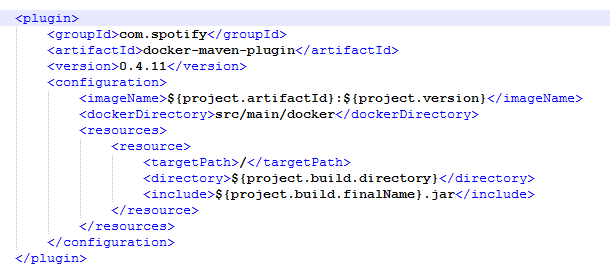
\includegraphics[width=\linewidth]{images/maven-plugin.PNG}
  		\caption{Maven Docker Plugin.}
  		\label{fig:docker-plugin}
	\end{figure}

\par
Om te connecteren met onze Cassandra cluster maken we gebruik van de Datastax java-driver. Datastax is een bedrijf dat een commerciële versie van Apache Cassandra aanbiedt alsook support voorziet. Hun Java-driver is open-source en dus gratis te gebruiken, in mijn ervaring biedt deze ook een betere ondersteuning voor het gebruik van UDTs tegenover de JPA-implementatie voor Cassandra. Om deze driver te gebruiken moeten we onze klassen die overeenstemmen met een tabel in onze databank annoteren met ‘@Table’. De velden in deze klassen krijgen nog de annotatie ‘@Column’ en ‘@PartitionKey’ als het gaat om een primary key kolom. De types van onze databank voorzien we ook klassen voor die we annoteren met ‘@Field’. De velden hier annoteren we met ‘@Field’. Eenmaal we onze tabellen hebben vertaald naar overeenstemmende klassen volstaat het om een sessie met onze cluster aan te maken, bij het aanmaken hiervan volstaat het om het IP-adres van één node te voorzien, de driver zal dan via discovery de locatie van de overige nodes vinden en zo fouttolerantie te waarborgen. Het is toch aan te raden om meerdere IP-adressen mee te geven zodat wanneer er een node niet beschikbaar is tijdens het aangaan van de sessie, deze kan terugvallen op een andere node.
\par
Verder voorzien we drie rest controllers: één voor elk hoofdmodel dat we hebben voorzien. Voor onze AEM-applicatie te kunnen voeden moeten we minstens twee endpoints per controller moeten voorzien, één voor het ophalen van de gewijzigde IDs per model en één voor het effectief ophalen van de data. 
	\subsection{Docker}
	De volgende stap is ons process is een manier zoeken om onze service in de cloud te draaien. Het is aanvaardbaar om tijdens de ontwikkeling onze service lokaal te draaien maar als we een volwaardig platform willen creeeren moet ook dit onderdeel remote draaien.
	\par
	\begin{wrapfigure}{r}{0.5\textwidth}
  	
\includegraphics[width=0.4\textwidth]{images/docker-logo.PNG}
	\end{wrapfigure}
	
	Docker is een open-source project dat dit process voor ons zal versimpelen. Vroeger moest er heel wat tijd (en bijgevolg ook budget) gespendeerd worden aan het werkende krijgen van services op verschillende machines. Dit komt omdat niet elke machine hetzelfde geconfigureerd is alles even goed ondersteund. Docker lost dit probleem op door maar één vereiste te hebben, dat de machine de Docker service heeft draaien. Oorspronkelijk ondersteunde enkel Linux systemen deze service native maar ondertussen zijn ook Windows en Mac mee op de kar gesprongen. Om deze lokaal te trainen, voor testing doeleinden, kan men naar de docker website gaat en de gewenste versie te downloaden. De tutorials die je daar kan vinden leggen perfect uit hoe je ermee aan de slag kan. Natuurlijk gaan we, na een korte uitlichting, onze Docker remote gaan draaien.
	\par
	Wie Docker zegt, zegt containers. Om onafhankelijk van de host een applicatie te kunnen draaien, steekt Docker deze, en al het nodige (environment, tools, libraries,settings,...), in een container. Docker bundelt al het nodige samen en maakt er een exporteerbare image van. Deze image kunnen we dan eender waar draaien zonder ons zorgen te moeten maken om infrastructurelen verschillen. Dit wil zeggen dat wanneer een image succesvol in een trainingsomgeving draait, deze zonder vrees overgezet kan worden naar een productie omgevening.
	\par
	Een ander voordeel van het containersysteem is dat men elke container, tijdens het opstarten, specifieke parameters kan meegeven met betrekking tot de resources die deze ter beschikking krijgt. Als men enkele zwaardere services heeft, kan met de container hiervan meer RAM toekennen dan anderen om aan de behoefte te voldoen. Het is perfect mogelijk om meerdere containers op één machine of verdeelt over meerdere machines te draaien wat de schaalbaarheid en beschikbaarheid ten goede komt. Zelfs een release hoeft geen downtime meer te betekenen, de containers kunnen één voor één vervangen worden met een nieuwere versie.
	\par
	Buiten de configuratie met betrekking tot de resources kan men ook omgevingsvariabelen meegeven (hoe dit mogelijk is zien we dadelijk). Dit heeft als voordeel dat we dezelfde container kunnen gebruiken voor onze trainings-en productieomgeving door ander variabelen, zoals de databaselocatie en credentials, urls van andere services, enz., mee te geven tijdens het starten van onze containers.
	\subsection{AWS en Docker}
	Nu wordt het tijd dat we onze services in de cloud gaan draaien. Hiervoor zijn enkele stappen nodig beginnend bij de installatie van de nodige software op onze ontwikkelings machine. De eerste installatie is die van de AWS Command Line Interface (of kortweg AWS CLI), gelukkig voor ons heeft Amazon hier een uitstekende handleiding\footnote{http://docs.aws.amazon.com/cli/latest/userguide/installing.html}
	voor. Het is belangrijk niet te vergeten om na de installatie deze ook te configureren\footnote{http://docs.aws.amazon.com/cli/latest/userguide/cli-chap-getting-started.html}.
	\par
	Het tweede wat we nodig zullen hebben is Docker op onze ontwikkelings machine, niet omdat we onze containers hier gaan draaien maar omdat we deze hier gaan bouwen. Voor diegene zonder ervaring met Docker raad ik deze manier aan om een beter begrip te krijgen van hoe dit in zijn werk gaat. De ervaren lezer mag natuurlijk zijn images op zijn gekozen manier bouwen. Om Docker te installeren kan de Linux-gebruiker zijn shell gebruiker, Mac en Windows hebben minder geluk en zullen een installer\footnote{https://docs.docker.com/engine/installation/} moeten gebruiken.
	\par
	Eenmaal onze ontwikkelings machine klaar is keren we terug naar AWS om een ECS-cluster (EC2 Container Service) op te zetten, hierin gaan we onze containers laten draaien. Een cluster kunnen we zien als een logische groepering van machines, wanneer we één dezelfde image meermaals deployen zullen de benodigde containers automatisch verdeelt worden over de machines in onze cluster.
	\par
	Voor we aan onze cluster beginnen maken we snel 2 IAM roolen aan, één rol voor onze machines en één rol voor de service die we op onze cluster zullen starten. De rol voor de machines geven we een logische naam: ecs-instance-role en geven we de permissie AmazonEC2ContainerServiceforEC2Role {Geeft de machine schrijfrechten op CloudWatch en ECS, leesrechten op ECR}. De rol voor de service noemen we ecs-service-role en geven we de de permissie AmazonEC2ContainerServiceRole (schrijf-en leesrechten op EC2 en ELB). 
	\par	
	 Een ECS cluster opzetten is geen werk, even navigeren naar scherm, kiezen om een nieuwe te maken, we geven deze een naam(bv. tst-ecs-cluster) en voor nu selecteren we de optie 'Create an empty cluster'. Als we nu een cluster aanmaken dan zien we deze verschijnen onder cluster verschijnen maar zonder instances in, deze toevoegen is een volgende stap.
	\par
	Vervolgens maken we een Launch configuration aan, dit zal beschrijven hoe onze machines opgestart moeten worden. De configuratie heeft als voordeel dat we dit maar eenmaal moeten doen en dat alle machines binnen onze cluster met de zelfde configuratie opstarten. DIt is grotendeels gelijk aan het maken van een machine, let wel op dat je als AMI\footnote{Amazon Machine Image} de Amazon ECS-optimized\footnote{te vinden onder AWS Marketplace} kiest. Dit zal onze machines automatisch van Docker voorzien en deze ook starten wanneer de machine boot. Ken ook de ecs-instance-rol toe aan onze machines bij de stap Configure details. In deze stap voegen we ook een script toe onder User data (Advanced Details). Hier schrijven we het script als gezien in Figuur \ref{fig:ecs-script}. Dit zal ervoor zorgen dat de machines die met deze configuratie starten aan onze cluster worden toegevoegd.
	\begin{figure}[h!]
		\centering
  		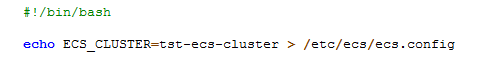
\includegraphics[width=0.5\textwidth]{images/ecs-script.PNG}
  		\caption{ECS bootup script.}
  		\label{fig:ecs-script}
	\end{figure}
	\par
	Nu we een Launch configuration hebben kunnen we deze gebruiken om effectief machines aan te maken. Dit doen we door een Auto Scaling Group aan te maken via de EC2 module. Tijdens het opzetten van deze groep kiezen we de Launch configuration die we juist hebben aangemaakt. We geven de groep een naam en hoeveel machines we willen bij de opstart ervan alsook een subnet, dit subnet kan gebruikt worden om strengere security filters in te stellen door enkel machines binnen dit subnet met elkaar te laten communiceren. Men zou dan via routing kunnen werken om een bepaald deel van de endpoints publiek toegankelijk te maken. In dit project gaan we hier niet verder op in. Onder Scaling Policies kunnen we beschrijven onder welke voorwaarden er meer machines moeten worden bijgezet, bijvoorbeeld als het CPU verbruik van onze cluster gedurende 5 minuten boven de 80\% is. Omgedraaid kunnen we ook instellen wanneer er machines verwijdert mogen worden buiten de piekuren. Als alles goed verlopen is zien we na creatie een aantal machines, gelijk aan het gekozen aantal, opstarten onder ons EC2 Instances scherm. Deze machines zouden, dankzij het ecs-script, ook te zien zijn als bij onze ECS-cluster gaan kijken onder Instances.
	\par
	Nu rest ons enkel nog het toevoegen van een loadbalancer en we zijn klaar om onze Docker containers te bouwen en te deployen naar onze nieuwe cluster. Een loadbalancer fungeert als gateway naar onze machines, inkomende requests op onze loadbalancer worden verdeelt en doorgestuurd naar de machines die de balancer als gezond beschouwt. Om de gezondheid van een machine te controleren doet deze periodiek een request naar de machines, zolang de machines met een status 200 antwoorden beschouwt de balancer ze als gezond. Hoe frequent en hoe vaak een antwoord positief of negatief moet zijn om de status van de machine te veranderen kan ingesteld worden. Ook de snelheid waarmee de machine moet antwoorden kan geconfigureerd worden, standaard is dit 5 seconden maar als je met gratis micro machines werkt verhoog je dit best. De netwerk capaciteiten van deze machines zijn beperkt waardoor de limiet van 5 seconden overschreven kan worden waardoor onze loadbalancer deze als ongezond zal beschouwen.
	\par
	
\end{document}


	
	\chapter{De scheduler}
	% !TeX spellcheck = nl_NL
\documentclass{article}

\begin{document}
	\section{Obsidian Scheduler}
	Obsidian is een Java-based scheduler waar een organisatie wederkerende jobs kan instellen. Obsidian is gratis in gebruik als je enkel alleenstaande instances hebt lopen, d.w.z. geen master-slave verhoudingen tussen instances.
	\par
	Om Obsidian te installeren hebben we een machine nodig waar reeds een Tomcat en databank op draait. Voor de database hebben we de keuze uit enkele populaire namen zoals MySQL en MS SQL. Wanneer aan deze twee vereisten zijn voldaan kunnen we de obsidian-x.x.x.jar downloaden en runnen met volgend commando. 
	\begin{lstlisting}
		$ java -jar Obsidian-Install-n-n-n.jar -console
	\end{lstlisting}
	Het '-console' zorgt ervoor dat we onze installatie zonder een UI kunnen configureren, hier vullen we onder andere in welke folder Obsidian terecht komt en de database gegevens. Eenmaal compleet hebben we een war in onze opgegeven folder gekregen, deze deployen we in onze Tomcat. Als we de default gegevens hebben laten staan kunnen we nu op poort 8080 van onze machine aan de UI van onze obsidian. We kunnen inloggen met de gebruiker admin en paswoord changeme.
	\par
	Onze installatie is voorzien van enkele standaard jobs maar het is mogelijk om via de Java API zelf jobs te coderen. De API voorziet de interface InterruptableJob die een klasse dwingt om de execute methode te implementeren, deze heeft een JobContext als parameter. Obsidian scant de lib folder van Tomcat en pikt de klassen die deze interface implementeren op als jobs. Om vanuit de UI parameters te kunnen meegeven moeten we onze klasse voorzien met de Configuration annotatie, hierin defini\"eren we een array van @Parameter annotaties. Elke parameter geven we een naam, een type, of deze vereist is en een eventuele default waarde. Tijdens het runnen van onze job kan je de parameterwaarde uit de JobContext halen.
	\par
	Voor dit project maken we twee jobs aan, \'e\'en die alle categorie\"en ophaalt en doorstuurt naar AEM en eentje die enkel de gewijzigde ophaalt. Beide jobs hebben twee stappen waarvan de eerste het ophalen van de categorie\"en is. De eerste job doet dit zonder parameter en krijgt alles binnen, de jog voor de gewijzigde doet dit met een datum en krijgt enkele die gemodificeerd zijn na deze datum binnen. De volgende stap is identiek voor de jobs, itereren over de opgehaalde categorieën en deze \'e\'en voor \'e\'en doorsturen naar AEM, dit zal het pagina generatie proces starten.
\end{document}	
	
	\chapter{Adobe Experience Manager}
	% !TeX spellcheck = nl_NL
\documentclass{article}

\begin{document}
	\section{Architectuur van AEM}
	In dit hoofdstuk gaan we de bouwstenen van AEM bekijken, de frameworks die worden gebruikt om de geboden functionaliteit mogelijk te maken en de interfaces die we ter beschikking krijgen om onze applicatie te beheren. De reden dat we dit doen is omdat deze ingebakken zijn in AEM, wie met AEM aan de slag gaat, zal ongetwijfeld met deze technologieën te maken krijgen. Het is aan te raden eerst deze sectie te lezen om een beter begrip te krijgen wat we doen en waarom we dit doen. We beginnen bij het open-source gedeelte en bekijken vervolgens waarvoor we betalen.

\end{document}
	% !TeX spellcheck = nl_NL
\documentclass{article}

\begin{document}
	\subsection{OSGi}
	OSGi (Open Services Gateway initiative) is een framework dat ons in staat stelt om Java applicaties uit verschillende modules op te bouwen. Deze modules worden bundels genoemd die onafhankelijk van elkaar geïnstalleerd, verwijdert en vervangen kunnen worden in een OSGi container. Een bundel bestaat uit de jars en resources nodig voor de interne werking van deze bundel. Tijdens het bundelen kan er gespecificeerd worden welke packages zichtbaar zijn voor de andere bundels, als we niets configureren zal geen enkele package publiek beschikbaar zijn. Dit is in contrast met de normale werking van jars waar elke jar op het classpath aan alle (publieke) klassen kan. Wanneer we een bundel installeren (of verwijderen) hoeven we de container niet stop te zetten. Dit geeft dat er geen down time is tijdens het updaten van onze applicatie.
	\par
	Omdat de bundels onafhankelijk van elkaar geïnstalleerd worden, kan een bundel niet rechtstreeks rekenen op klassen voorzien door een andere bundel. Indien bundels toch afhankelijk zijn van elkaar worden er interfaces voorzien die geregistreerd worden in een service laag. Stel dat bundel A een externe StoreService gebruikt om een winkel te kunnen ophalen, zolang deze interface geregistreerd is in de service laag kan onze bundel starten zonder probleem. Wanneer bundel B start met een implementatie van StoreService (bv. StoreServiceImpl), kunnen we deze registreren in de service laag. Bundel A luistert naar veranderingen in de service laag en zodra StoreServiceImpl beschikbaar is, zal deze in gebruik genomen worden. In het geval dat bundel B verwijdert word, zal deze ongeregistreerd worden en zal bundel A hiervan op de hoogte zijn.
	\subsection{Apache Felix}
	Apache Felix is de open source OSGi-container van Apache en wordt gebruikt door AEM voor het installeren van de bundels die onze componenten bevatten. In deze container zullen onze bundels draaien en met elkaar communiceren om samen de applicatie van zijn functionaliteit te voorzien.
\end{document}
	% !TeX spellcheck = nl_NL
\documentclass{article}

\begin{document}
	\subsection{JCR en Apache Jackrabbit}
	De Java Content Repository API (JCR) is een api die gebruikt kan worden om data op te slaan in een boomstructuur. Deze boom bestaat uit twee zaken: nodes en properties, nodes vormen de toppen van onze boom waardoor we kunnen navigeren, de top van onze bomen heet de rootnode. De properties zijn de blaadjes van onze toppen die effectieve data bevatten zoals een stuk tekst of getallen. We kunnen door onze nodes navigeren aan de hand van de methodes die de api beschikbaar stelt, we kunnen nagaan of onze node kinderen heeft en hoe deze heten alsook onze ouder bekijken. De data structuur van onze nodes kunnen we definiëren aan de hand van een type. Dit type kan gebruikt worden om bepaalde velden af te dwingen alsook restricties omtrent de toegestane velden op te leggen. Dit type kan ook indiceren dat alles is toegestaan. 
	\par
	In functie van een CMS applicatie kunnen we onze boom beschouwen als de data op onze pagina's. Onze rootnode is onze homepage en diens kinderen vormen onze navigatie, wanneer we naar de pagina merken navigeren bewegen we ons vanaf onze rootnode naar diens kind 'merken'. De kinderen van de node 'merken' stellen dan elk een effectief merk voor. Omdat de data ongestructureerd is hoeft niet elk merk dezelfde properties te bevatten, tijdens het generen van de pagina kunnen we zaken tonen, of juist niet, aan de hand van de aanwezigheid van bepaalde properties. Dit is een voorbeeld om aan te tonen hoe je met JCR een website kunt opbouwen.
	\par
	Het is belangrijk om te begrijpen dat het niet de bedoeling is om traditionele data op te slagen in JCR, enkel content. Apache Jackrabbit is Apaches implementatie van JCR en is geïntegreerd in Apache Sling.
\end{document}
	
	\subsection{Apache Sling}
	Sling is een framework van Apache dat de gebruiker in staat stelt om REST calls te doen via HTTP. Het ondersteunt verscheidene bestand types waaronder JSON, XML en HTML. Sling is het framework dat AEM gebruikt om aan de hand van een URL van een request de juiste node te vinden en diens data terug te geven in de correcte vorm. Door een extensie mee te geven kunnen we aan Sling duidelijk maken hoe we onze data willen, bv. door \textquotedbl .json\textquotedbl{} achteraan een URL toe te voegen, weet Sling dat we de data als JSON terug willen.
	\par
	Sling is reeds ge\"integreerd met zowel Apaches Jackrabbit alsook Felix waardoor het de eigenschappen van beiden heeft. Dit wil niet zeggen dat JCR de enige manier is om met Sling data op te slaan, indien gewenst kan er ook met andere databanken zoals SQL of MongoDB gewerkt worden. 
	\par
	 Wanneer een Sling bundel ge\"installeerd wordt, registreert het een ResourceProviderFactory bij de service laag van onze OSGi container.  

	% crx is deel author 
	% !TeX spellcheck = nl_NL
\documentclass{article}

\begin{document}
	\subsection{Author}
	\subsubsection{CRX}
	Nu we de open source onderdelen van AEM hebben gezien is het tijd om de gelicentieerde delen bespreken. Het eerste dat we bespreken is Adobe CRX wat, simpelweg gezegd, Adobes implementatie is van Apache Jackrabbit en Sling. Buiten alle features die deze frameworks bieden heeft Adobe bijkomende functionaliteit toegevoegd, anders zou het maar raar zijn om hiervoor te betalen. We bekijken kort diegene die we gebruiken tijdens dit project.
	\par
	Zoals we reeds gezien hebben is de datastructuur van JCR een boom waarin we kunnen navigeren. Een feature die CRX voorziet is een UI waarmee we kunnen navigeren door onze nodes, de CRXDE. Met deze interface kunnen we onze nodes bekijken zoals we een filesystem zouden gebruiken. We kunnen nodes expanderen en hun kinderen bekijken om ook deze te expanderen en zo dieper in onze boom af te dalen, of we kunnen de properties van de node zelf bekijken. De kracht van deze UI is dat we een gestructureerd overzicht van de nodes zien die onze website vormgeven.
	\par
	De package manager is een ander belangrijk onderdeel van de CRX en geeft ons de optie onze packages te beheren. Via deze UI kunnen we packages toevoegen, verwijderen en installeren. Wanneer een package wordt ge\"installeerd, worden diens OSGi bundels opgemerkt en actief in de OSGi container. Het is belangrijk te beseffen dat eenmaal een bundel in de container leeft, de package manager hier geen invloed meer op heeft. Indien, na installatie, een package wordt verwijderd, blijft de corresponderende OSGi bundel actief. Om deze bundel te verwijderen moeten we ons wenden tot de OSGi console.

\end{document}
	% dit is de editor, deel author 
	
	\subsubsection{Editor}
	Alles wat we tot hiertoe gezien hebben heeft als functie het voorzien van componenten die bepaalde functionaliteit bezitten. Eenmaal we de componenten ontwikkeld hebben en via onze bundels ge\"installeerd zijn, is het tijd voor de designers aan de slag te gaan. De belangrijkste feature van AEM is de mogelijkheid om content te voorzien, gebruik makend van onze componenten. We kunnen deze slepen op templates, configureren en voorzien van inhoud. Een marketeer kan zo een volledige pagina, inclusief de navigatie hiernaar toe, opbouwen zonder een enkele HTML tag of Javascript regel te schrijven. Wanneer een pagina af is, kan men deze ook publiceren via AEM zodat het resultaat door de wereld gezien kan worden.
	\subsubsection{DAM}
	De DAM (Digital Asset Manager) is een opslag plaats waar we onze verschillende media kwijt kunnen zoals foto's of video's. Eenmaal opgeslagen in de DAM kunnen we deze gebruiken op onze website door middel van referentie, later zien we hoe dit praktisch in zijn werk gaat.
	\subsubsection{Een author opzetten}
	Voor het opstarten van een author heb je twee zaken nodig: de quickstart jar en een license.properties file, beiden te verkrijgen via de Adobe website. Indien we deze ter beschikking hebben, plaatsen we deze in een folder \textquotedbl author\textquotedbl{} en voeren de jar uit met volgend commando (dit is voor een 64bit machine).
	\begin{lstlisting}
		 $ java -XX:MaxPermSize=256m -Xmx1024M -jar cq5-author-p4502.jar
	\end{lstlisting}	
	\par
	Met dit commando start de author op poort 4502 van de machine, om te verifi\"eren dat het opstarten succesvol is verlopen, surfen we naar \textquotedbl http://ip-van-de-machine:4502/projects\textquotedbl{} in onze browser. Dit opent de UI van de author waarbij we, onder andere, kunnen bekijken welke sites er reeds zijn. Als je de jar zonder parameters hebt gestart zouden er al enkele voorbeelden gedefini\"erd moeten zijn. Met de standaard instellingen zal de author naar een publisher zoeken op poort 4503 van dezelfde machine om zijn wijzigingen naar toe te pushen.

	% !TeX spellcheck = nl_NL
\documentclass{article}

\begin{document}
	\subsection{De publisher}
	\subsubsection{Het nut van een publisher}
	Een publisher is niet meer dan een afgeslankte author, alle management en editor tools zijn weggenomen en enkel de repositories worden bijgehouden. Dit zorgt dat marketeers geen pagina's kunnen editeren op een publisher maar dat deze wel in staat is om pagina's te genereren. Omdat een AEM-licentie restricties legt op het aantal authors maar niet op de publishers is dit een manier om de load op de author te verminderen. Normaal zou de author voor elk request een pagina generen maar dit kan uitbesteed worden aan \'e\'en of meer publishers waardoor deze zich kan focussen om het content management gedeelte.
	\par
	Voor een publisher een request kan afhandelen moet deze weet hebben van de content op de website. Hiervoor heeft een publisher een kopie van alle noden in een persoonlijke JCR-repository. Elke publisher is bij de author geregistreerd als een agent, wanneer er een pagina opnieuw wordt gepersisteerd wordt deze pagina naar elke publisher verzonden zodat deze up-to-date blijven met de author. Een binnenkomend request heeft hierdoor altijd hetzelfde resultaat ongeacht de publisher die deze verzorgt.
	\subsubsection{Een publisher opzetten}
	Om een publisher op te zetten gaan we hetzelfde te werk als bij de author, we maken een folder "publish" met wederom onze jar en licentie in, de jar moeten we hernoemen. We vervangen "author" door "publish" en de poort passen we aan naar 4503 wat resulteert in het volgende commando.	
	\begin{lstlisting}
		 $ java -XX:MaxPermSize=256m -Xmx1024M -jar cq5-publish-p4503.jar
	\end{lstlisting}
	 Dit start een publisher op poort 4503, het verschil is dat deze geen editor ter beschikking stelt, we kunnen enkel onze website opvragen.
\end{document}
	% !TeX spellcheck = nl_NL
\documentclass{article}

\begin{document}
	\subsection{Dispatcher}
	De dispatcher is AEM's eigen caching laag en dient als publieke gateway voor de gebruikers. Doordat de publieke requests via de dispatcher gaan voorziet deze een extra beveiligingslaag. Dit door het feit dat we AEM kunnen afschermen voor requests van buiten ons netwerk. Om een dispatcher op te zetten installeren we de module op een web server en configureren deze. Deze configuratie bevat, onder anderen, waar onze AEM draait, welke soort bestanden er gecached moeten worden en hoe de cache van deze bestanden vervalt.
	\par	
	 Wanneer een dispatcher een request binnen krijgt wordt deze eerst geanalyseerd of deze in aanmerking komt voor onze cache. Buiten onze configuratie zijn er ook enkele standaard regels waarna gekeken wordt om dit te bepalen. Enkel de HTTP methode GET komt in aanmerking voor de cache, indien het request een andere methode bevat kan deze niet gecached worden. Ook wanneer er een request parameter wordt meegegeven kan de request niet gecached worden aangezien zo'n request een variabel antwoord heeft.
	\par
	Er zijn vier manieren waarop een cache kan vervallen, de eerste zijnde een levensduur aan de caches toekennen. Wanneer een cache deze levensduur overschrijdt vervalt deze, bij een volgend request wordt er een nieuwe call naar de publisher gedaan. Deze nieuwe versie vervangt vervolgens de oude cache en wordt naar de gebruiker doorgestuurd.
	\par
	Een andere mogelijkheid is om de cache van een pagina te verwijderen wanneer een nieuwe versie beschikbaar wordt. Hiervoor moet de author een flush request doen naar de dispatcher toe op het moment dat een pagina wordt gepublished. Dit request verwijdert de cache, de volgende keer dat de pagina wordt opgevraagd is de dispatcher verplicht om deze opnieuw op te halen.
	\par
	 Een andere manier om bij het publiceren een cache te invalideren is met het gebruik van stat bestanden. Een stat bestand is een record dat (onder andere) de laatste datum van modificatie onthoudt. Wanneer een pagina wordt gepubliceerd, plaats de author een stat bestand voor deze pagina op de dispatcher. Het tijdstip van modificatie van het stat bestand zal telkens vergeleken worden met die van de gecachte pagina. Indien die van de pagina ouder is, weet de dispatcher dat er een nieuwe versie beschikbaar is. Vervolgens verwijdert de dispatcher de cache en haalt de nieuwe versie op.
	 \par
	 Een laatste techniek is het expliciet verwijderen van de bestanden op de dispatcher. Deze zal niet meer in staat zijn de pagina terug te vinden en wordt verplicht om deze opnieuw op te halen. Dit kan manueel gebeuren door in te loggen op de machine of via een script dat periodiek wordt uitgevoerd.
\end{document}

	\chapter{Omgaan met dynamische data}
	% !TeX spellcheck = nl_NL
\documentclass{article}

\begin{document}
	\section{Een eerste project}
	In de vorige hoofdstukken hebben we services voorzien die data op verscheidene manieren kunnen ophalen, het enige wat nog ontbreekt is een applicatie om deze te gebruiken. In dit deel gaan we onze eerste AEM applicatie bouwen en proberen we de verschillende manieren uit om deze applicatie van data te voorzien.
	\subsection{Een author lokaal draaien}
	Tijdens het ontwikkelen van een AEM-applicatie is het aangeraden om een lokale author te draaien. We kunnen deze omgeving gebruiken om onze geschreven componenten een eerste keer in actie te zien zonder deze op een remote server te moeten deployen. Voor het opstarten van een author heb je twee zaken nodig: de quickstart jar en een license.properties file, beiden te verkrijgen via de Adobe website. Indien we een geldige licentie hebben kunnen we author starten door simpelweg de jar te runnen.
	\par
	Standaard start de author op poort 4502 van onze machine, om te verifiëren dat het opstarten succesvol is verlopen surfen we naar http://localhost:4502/projects in onze browser. Dit opent de UI van de author waarbij we, onderhanden, kunnen bekijken welke sites er reeds zijn. Als je de jar zonder parameters hebt gestart zouden er al enkele voorbeelden gedefinieerd moeten zijn. Natuurlijk zijn we hier niet in geintreseed en gaan we zelf een website opzetten. De website, en bijhorende componenten, kan je rechtstreeks via deze UI aanmaken maar is niet aan te raden. De mogelijkheden zijn beperkt en er is geen spraken van versie beheer, voor ons project gaan we een andere aanpak gebruiken.
	\subsection{Een Maven project aanmaken}
	\begin{wrapfigure}{l}{0.5\textwidth}
  		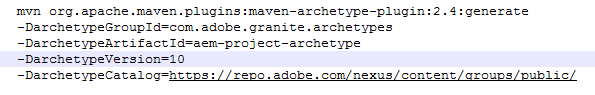
\includegraphics[width=0.4\textwidth]{images/maven-archetype.PNG}
	\end{wrapfigure}
	Het gebruiken van een Maven project heeft verscheidene voordelen: we kunnen rest endpoints voorzien die men kan gebruiken om data naartoe te sturen (pagina's generen), business logica ontwikkelen in de vorm van Java-klassen en we kunnen het project beheren via git waardoor we een historiek van aanpassingen hebben. Het handmatig aanmaken van zo'n project kan lastig zijn, gelukkig voor ons heeft Adobe een template project voorzien die we kunnen gebruiken.
Wanneer we volgend commando uitvoeren (vereist Maven versie 3.3.1 of hoger) wordt ons gevraagd om enkele zaken te specificeren zoals de naam van onze website, de naam van onze modules en OSGi-bundels. Wanneer deze zijn ingevuld wordt het project aangemaakt en kunnen we aan de slag gaan.
	\subsection{Structuur van het Project}
	Wanneer we het project openen zien we dat de template voorzien is van meerdere modules die elk dezelfde prefix maar andere suffix hebben, we overlopen kort de belangrijksten. De core-module bevat onze Java-klassen: repositories,dto's, rest controllers, onze modellen, enz. De ui.apps-module bevat het frontend gedeelte: de html, CSS, JavaScript, templates, enz. De ui.content-module bevat onze effectieve website, wanneer we deze deployen worden alle pagina's vervangen door wat er zich in deze module bevindt. Als onze Maven profielen ongewijzigd zijn gebeurt dit samen met het deployen van de ui.apps-modulen (dus wanneer we onze componenten bundel uploaden). Vanzelfsprekend willen we niet bij elke deploy alle pagina's van onze website verwijderen dus splitsen we deze uit naar een ander profiel. Voor het coderen van componenten houden we ons voornamelijk bezig met de core en ui.apps-module.
	\subsection{Een component maken}
	Voor wie nog geen ervaring heeft met het aanmaken van componenten via een Maven project kan het moeilijk zijn om het doel van elk bestand te achterhalen, bijkomend is de documentatie schaars en vooral gericht op het werken met de author. In dit stuk gaan we een simpele component aanmaken en verklaren we wat waarvoor dient.
	\par
	\begin{wrapfigure}{l}{0.5\textwidth}
  		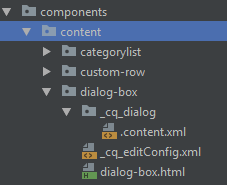
\includegraphics[width=0.4\textwidth]{images/component-pck-structure.PNG}
	\end{wrapfigure}
	Een component bestaat uit verschillende files gedefinieerd onder een folder die de naam van de component draagt. Ter illustratie maken we een dialog-box component, als eerste maken we de folder aan. In deze folder definiëren we een dialog-box.html wat de structuur zal beschrijven. Als basis gebruiken we een Bootstrap panel waarbij we een titel en een tekst kunnen invullen. Vervolgens voegen we een \_cq\_editConfig.xml wat ons toelaat te definiëren hoe deze component gebruikt kan worden, enkele voorbeelden zijn: of deze via de author mag versleept worden, of de inhoud gewijzigd kan worden en op welke type pagina's deze component geplaatst kan worden. Als laatste hebben we een .content.xml, hierin kunnen we specificeren wat er aan de component kan meegegeven worden wanneer deze op een pagina wordt gesleept. In ons voorbeeld voorzien we drie zaken: een titel, een tekst en een grote.
	\begin{figure}[h!]
  		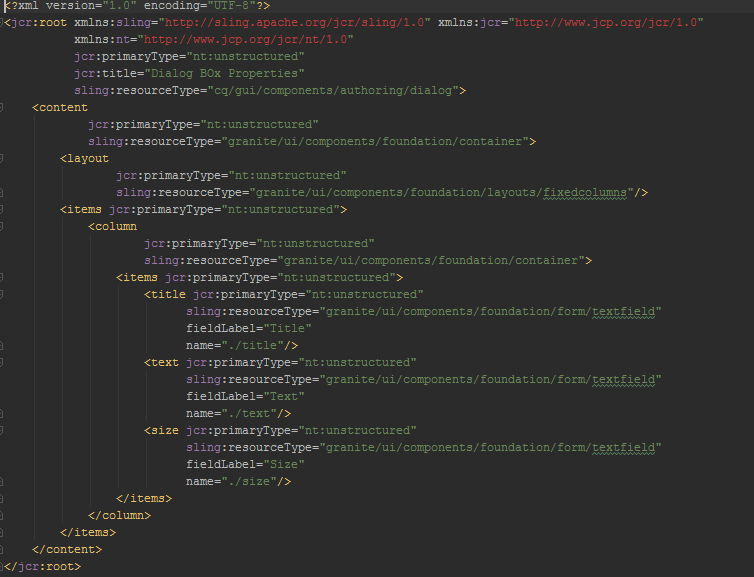
\includegraphics[width=\linewidth]{images/content-xml.PNG}
  		\caption{.content.xml}
  	\end{figure}
	\par
	We kunnen ook een Java-klasse voorzien waarop we de velden van de .content.xml kunnen injecteren. De Java klasse werkt als placeholder voor de velden van onze paginanode, als we een property '<custom-tag>:title' hebben voorzien we hiervoor een String en annoteren die met @Inject en @Named('<custom-tag>:title'). Dit maakt het mogelijk om fallbacks in te bouwen alsook extra logica te voorzien, bv. een service gebruiken om data op te halen die we in onze html willen gebruiken.  
	\par
	Nu is het mogelijk om via Sightly onze klasse te koppelen aan onze html door het attribuut 'data-sly-use.dialogBox="<package naam>.<klasse naam>"' in een html tag toe te voegen. Het stuk na 'data-sly-use.' definiëert hoe we deze gaan aanspreken, in ons voorbeeld hebben we deze dialogBox genoemd. Nu kunnen we binnen de html tag onze klasse gebruiken via volgende syntax: \${dialogBox.title}, gegeven er een getTitle() methode op onze Java-klasse staat.

\end{document}
	% !TeX spellcheck = nl_NL
\documentclass{article}

\begin{document}
	\subsection{Pagina's genereren} 
	\subsubsection{Wat is het?}
	Als we pagina's gaan genereren, gaan we wijzigingen van het ERP doorduwen naar AEM. AEM gaat aan de hand van deze informatie noden aanmaken in onze JCR repository en per taalvariant een pagina voorzien. Eenmaal de pagina's aangemaakt zijn, kunnen ze via de corresponderende url worden opgehaald.
	\subsubsection{Hoe werkt het?}
	Om deze optie te voorzien moeten er enkele zaken gecodeerd worden in Java, met name de functionaliteit om via de SlingRepository de data weg te schrijven naar een node en de PageManager van AEM gebruiken om de pagina's aan te maken. Alsook moeten we een HTML template voorzien die we kunnen gebruiken om onze categorie weer te geven. Tijdens het genereren van de pagina kunnen we verwijzen naar deze template om een standaard look te geven aan de pagina. Eenmaal deze pagina er is kan het contentteam aan de slag om deze een persoonlijke touch te geven.
	\par
	Om een node aan te maken moeten we eerst een Session verkrijgen waarin we kunnen werken, dit kunnen we doen door de login methode op onze SlingRepository aan te roepen met onze credentials. JcrUtils is een voorziene klasse waarmee we noden kunnen aanmaken, hetgeen we nodig hebben is een pad waaronder we deze willen opslaan, het type dat we aan de node willen toekennen en onze reeds verkregen sessie. Als we de node hebben aangemaakt rest ons nog het over mappen van de velden naar onze noden, indien ons model velden bevat die een klasse op zich zijn, moeten we met geneste noden werken. Dit nesten heeft geen beperkingen en kan zo diep als nodig gaan. Het is aan te raden om deze velden te voorzien met een prefix om een duidelijk onderscheid te maken dus de properties die we zelf creëeren en diegene die door JCR aangemaakt zijn. Stel dat we een veld 'title' hebben die we wensen op te slaan, doen we dit onder '<custom-tag>:title'. Wanneer de velden zijn overgezet mogen we niet vergeten om de save methode van onze sessie aan te roepen zodat onze data gepersisteerd wordt.
	\par
	De volgende stap is een pagina voor ons model aanmaken, dit per taal waarin onze website beschikbaar is. Een pagina aanmaken gebeurt op een gelijkaardige manier als een node. We gebruiken de PageManager die de AEM api ons beschikbaar stelt. Omdat we zaken gaan persisteren moeten we ook hier werken met een sessie. Via de pageManager kunnen we onze root pagina van de website opvragen. De directe kinderen van deze pagina stellen de talen voor waarin onze site beschikbaar is. We itereren over deze lijst waarbij we per kind (lees taal) een pagina genereren. We maken deze pagina niet rechtstreeks onder de taalpagina aan maar voorzien een tussen pagina, bv. categoriëen. Wanneer we een categorie met id 14 hebben gaan we de pagina hiervoor opslaan onder <onze site>/nl/categorieen/14. Het pad dat we dan meegeven aan de create methode van de pageManager is het pad van de ouder waaronder we een pagina willen maken. Naast deze parameter geven we ook de pagina naam mee (in ons voorbeeld 14), de template (de locatie van de html die we gebruiken om onze pagina te tonen) en een modeltitel (bv. 'category'). Nu de pagina is aangemaakt kunnen we hiervan de node opvragen en kunnen we, conform aan vorige paragraaf, deze voorzien van properties. Ook hier prefixen we best onze namen.
    \par
    In vorige paragraaf gebruiken we een template om onze categorie te tonen, deze gaan we zelf voorzien. Het is best om hier gebruik te maken van het componenten systeem waarvoor AEM gekend is. In plaats van een specifieke html te coderen gaan we deze opslitsen in herbruikbare componenten. Hoe we componenten bouwen hebben we reeds gezien in een vorig hoofdstuk.
    \par
    Eenmaal we de nodige componenten hebben aangemaakt kunnen deze gebruikt worden om een template te voorzien. We kunnen de componenten rechtstreeks aan onze template toevoegen of een tussen component voorzien die kleinere componenten combineert. Dit kan handig zijn wanneer de zelfde combinatie van componenten meermaals gebruikt wordt (denk maar aan een navigatie), ook de css en js bestanden kunnen we in deze wrapper inladen zodat we ons daarover geen zorgen moeten maken wanneer we templates samenstellen. Eenmaal de template af is kan deze gebruikt worden om automatisch pagina's te genereren of om via de author handmatig een pagina toe te voegen.
	\subsubsection{De voordelen}
    Het voordeel van deze manier van werken is dat wanneer een gebruiker de pagina opvraagt, deze reeds voorzien is van data waardoor er geen repositories worden aangesproken. Uiteraard is dit wel het geval als we componenten toevoegen die dynamische content voorzien maar de properties die we aan onze node hebben toegevoegd zijn reeds aanwezig
    \par
     Een bijkomend voordeel is dat, door het feit dat er een pagina aangemaakt is, we deze via de author kunnen bewerken. We maken weliswaar een pagina via een standaard template maar hier hoeft het niet bij te blijven. We kunnen deze via de author gaan editeren en van specifieke content zoals een achtergrond afbeelding, een paragraaf met extra informatie of een uitgelicht product voorzien. Pagina's genereren is de enigste manier van werken die dit mogelijk maakt.
	\subsubsection{De nadelen}
    Het grote nadeel van deze methode is dat dit een vrij intensieve operatie is en het genereren zelden beperkt is tot één enkele pagina, wanneer een site drie talen heeft zal AEM telkens drie pagina's aanmaken. Dit wordt nog eens geëxpandeerd indien men via een blueprint werkt. Stel dat we een .com site hebben met drie talen, een .be site met drie talen en een .nl site met twee talen. Dit betekent dat per categorie AEM zeven pagina's moeten voorzien. Voor een model waar relatief weinig wijzigingen aan gebeurt is dit doenbaar, zoals ons categorie voorbeeld. Maar als we dit willen doortrekken naar producten, waar er mogelijks duizenden per dag wijzigen, is dit niet houdbaar. Onze author zou continue belast worden met het genereren van pagina's en potentieel bezwijken onder de load. Een tweede author plaatsen is zelden een optie omdat dit een tweede licentie vereist.
\end{document}
	
	\subsection{Een generieke pagina voorzien van data} 
	\subsubsection{Wat is het?}
    Voor sommige modellen is de vorige techniek niet haalbaar omwille van het feit dat dit zou resulteren in het genereren van een te groot aantal pagina's. Voor deze modellen is er een andere techniek beschikbaar, één pagina (al dan niet per taal) voorzien die we op het laatste moment gaan parsen met de bijhorende data. Ter illustratie beschouwen we de producten, dit kunnen er tienduizenden zijn waardoor de techniek van het genereren uitgesloten wordt (wegens de vermelde nadelen). In plaats daarvan gaan we een generieke pagina aanmaken die we voorzien met de productdata op het moment dat een gebruiker deze opvraagt. 
	\subsubsection{Hoe werkt het?}
    Als eerste hebben we een SlingFilter nodig, deze bekijkt alle binnenkomende request en manipuleert deze indien nodig. Om deze filter te maken voorzien we een Java-klasse van de annotatie in Figuur \ref{fig:sling-filter} en laten deze klasse de javax.servlet.Filter interface implementeren. De meegegeven scope vertelt Sling waar deze filter op werkt, in deze situatie willen we dat elk binnenkomend request deze filter passeert. De \textquotedbl order\textquotedbl{} property geeft aan in welke volgorde de filters moeten uitgevoerd worden indien er meerdere zijn. Hoe lager dit getal hoe eerder de filter aan bod komt.
    
    \begin{figure}[h!]
  		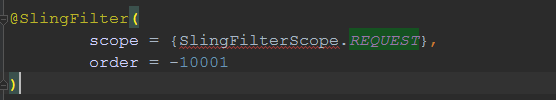
\includegraphics[width=0.8\textwidth]{images/sling-filter.PNG}
  		\label{fig:sling-filter}
	\end{figure}
	
    De Filter interface dwingt ons om drie methoden te implementeren, de init methode wordt uitgevoerd wanneer de filter in gebruik wordt genomen. De destroy methode is actief wanneer een filter wordt opgekuist, hierin kan men eventuele threads afsluiten of resources vrijgeven. Deze twee methodes laten we leeg en we focussen ons op de derde, de doFilter methode. Deze gaat elk binnenkomend request onder de loep nemen en deze (indien gewenst) manipuleren. Voor onze producten gaan we de url van een request bekijken, indien deze het patroon \textquotedbl /product/\textquotedbl{} bevat, weten we dat deze naar een product pagina moet leiden. We onderscheppen deze requests en sturen deze door naar de generieke product pagina. Voor het redirecten gebeurt gaan we eerst het product ID uit de url halen. Dit ID gebruiken we om (via een REST call) het bijhorende product op te halen en toe te voegen aan het binnengekomen request.
    \par
    De volgende stap is het voorzien van de generieke pagina, dit gebeurt grotendeels conform aan wat we al hebben gezien. We voorzien een HTML met daarop enkele componenten die gebruik maakt van een controller klasse. Het verschil met het reeds geziene is de soort controller dat we gebruiken, voorheen luisterde deze naar een node maar die hebben we deze keer niet. In plaats daarvan willen we de request beschikbaar stellen, daarop staat immers onze product informatie. Om hieraan te kunnen, voorzien we onze controller met de annotatie uit Figuur \ref{fig:request-controller}.

    \begin{figure}[h!]
  		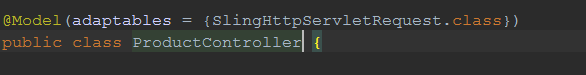
\includegraphics[width=0.8\textwidth]{images/request-controller.PNG}
  		\label{fig:request-controller}
	\end{figure}
    
    Het verschil met een controller voor een node zit in de \textquotedbl adaptables\textquotedbl{} waarde, voorheen was dit een resource. Door deze waarde te wijzigen weet Sling dat deze controller naar een request moet luisteren. Nu kunnen we via de \textquotedbl @Self\textquotedbl{} annotatie ons SlingHttpServletRequest ter beschikking stellen. Via de getAttribute methode kunnen we het product opvragen en gaan gebruiken voor bv. de getTitle methode van onze controlleren. 
	\subsubsection{De voordelen}
    Binnen AEM hoeven we maar \'e\'en product pagina te voorzien voor alle producten, in tegenstelling tot het genereren van pagina's. Dit zorgt dat deze techniek de author niet belast. Wanneer een product wijzigt gebeurt er niets totdat diens pagina wordt opgevraagd. Zelfs het opvragen veroorzaakt geen load op de author, het ophalen van de product date en het parsen van de HTML valt onder de verantwoordelijkheid van de publisher.
	\subsubsection{De nadelen}
    Het nadeel is dat deze techniek het moeilijker maakt om gepersonaliseerde product pagina's te voorzien. Een wijziging van de layout op de generieke pagina heeft een rechtstreeks effect op alle producten die deze gebruiken. Men kan hier rond werken door meerdere generieke pagina's te voorzien en op basis van het product naar een specifieke te redirecten. Zo kan men groepen van producten een ander uitzicht geven.
    \par
    Een ander (miniem) nadeel is de afhankelijkheid van REST services, als deze falen kan de data niet worden opgehaald en bijgevolg de pagina niet getoond worden. In deze proef ligt het beheer van deze services bij ons en zal downtime onwaarschijnlijk zijn. Wanneer men met externe services werkt, kan men beter een fallback inbouwen in het geval dat deze onverwacht offline gaan.

	% !TeX spellcheck = nl_NL
\documentclass{article}

\begin{document}
	\subsection{Server Side Includes} 
	\subsubsection{Wat is het?}
	SSi is een scriptingstaal die de mogelijkheid biedt om data in een bestaande html-pagina te injecteren. Deze injectie kan een effectief bestand betreffen maar kan evengoed een functie zijn, bv. de huidige datum ophalen. Vlak voor het versturen van de html zal de webserver alle SSI commando's opsporen en omzetten naar gewone html. De bestandtypes die men via SSI ophaalt kan verschillende vormen aannemen waaronder Json (bv. het resultaat van een rest call) en html (bv. een footer die ge\"injecteerd wordt). In het geval van Json zou men het resultaat kunnen gebruiken voor een javascript functie, bij html kan deze rechtstreeks worden afgebeeld. Best practice is om de SSI commando's in commentaar te zetten zodat deze verdwijnen wanneer de webserver SSI niet ondersteund.
	\subsubsection{Waarom SSI?}
    Binnen AEM kunnen we templates bouwen aan de hand van bestaande componenten, een goed voorbeeld is een template die een navigatie bevat, we willen immers op de meeste pagina's onze navigatie tonen. Wanneer deze template gebruikt wordt genereren we een pagina met daarop onze navigatie en een gespecifieerde inhoud. Als een gebruiker deze pagina ophaalt passeert dit verzoek de dispatcher, als de pagina nog in zijn cache zit kan deze onmiddelijk worden weergegeven. Indien dit niet het geval is moet deze opgehaalt worden bij een publisher, vervolgens wordt deze op de dispatcher gecached en doorgestuurd naar de gebruiker. Dit betekent dat de hele pagina, inclusief navigatie, gecached wordt op de dispatcher. 
    \par
    Zolang de navigatie ongewijzigd blijft brengt dit geen problemen te weeg. Stel nu dat er een nieuwe categorie aangemaakt wordt en deze zichtbaar moet worden in de navigatie. We hebben in het vorige hoofdstuk gezien hoe we categorie pagina's kunnen maken en hoe de navigatie deze oppikt. Het enige obstakel om deze live te krijgen is de dispatcher die de navigatie op elke pagina apart heeft gecached. We kunnen wachten tot deze verloopt maar dit tijdstip is voor elke pagina anders. Langzaam aan zullen de gecachte pagina's verlopen waardoor deze opnieuw moeten worden opgehaald (met de nieuwe navigatie). Tijdens deze overgangsperiode zal de navigatie op onze website inconsistent zijn, sommige pagina's hebben de oude (gecachte) versie en andere hebben reeds de nieuwe.
    \par
    Sommige lezers zullen nu denken: \"We kunnen toch de hele cache tegelijk invalideren? Dan moet de dispatcher wel de nieuwe versie ophalen.\". Deze gedachtegang is correct maar heeft \'en\'en groot nadeel: de publisher moet dan mogelijk enkele honderden pagina's tegelijk genereren wat kan leiden tot een crash. Buiten piekuren en met een beperkt aantal pagina's kan deze methode haalbaar zijn, voor een internationale enterprise applicatie is dit niet realistisch en moet er een andere oplossing gezocht worden.
    \par
    Deze oplossing kan men bekomen met het gebruik van SSI, in plaats van onze template rechtstreeks van de navigatie component te voorzien gebruiken we SSI om deze toe te voegen. Als men nu een pagina opvraagt zal de dispatcher deze laten genereren door de publisher maar deze zal de SSI-tag nog niet resolven. Deze tag wordt mee gecached, met de rest van de pagina, en zal pas op het laatste moment ervoor zorgen dat de navigatie wordt ge\"injecteerd. Wanneer deze injecte moet gebeuren zal de dispatcher de navigatie opvragen bij de publisher en deze cachen. Alle pagina's gaan nu de gecachte versie van onze navigatie injecteren en als deze wijzigt volstaat het om enkel de cache van de navigatie te invalideren.
    \par
    Het is belangrijk om te bezeffen dat SSI enkel op de dispatcher zal worden uitgevoerd wat geen probleem vormt in productie, elk request passeert hier. Voor het contentteam vormt dit wel een probleem, zij werken op de author en aangezien deze de injectie niet gaat uitvoeren zullen zij de navigatie niet te zien krijgen tijdens het editeren van pagina's. Een mogelijkheid is om overal waar men SSI wil gebruiken deze tag in een IF-statement te incapsuleren, indien de pagina niet vanop de author wordt opgevraagt gebruikt men de tag, anders injecteert men de data rechtstreeks.
	\subsubsection{De nadelen}
    E\'en nadeel hebben we reeds gezien, om het editeren van pagina's aangenaam te houden moeten we overal waar we SSI willen gebruiken extra statements voorzien om hetzelfde resultaat op de author te bekomen. Bij uitbundig gebruik kan dit leiden tot onoverzichtelijke code die moeilijk te onderhouden is.
    \par
    Een ander nadeel is dat de commando's worden uitgevoerd vlak voor de webserver de html verstuurd. Dit heeft als gevolg dat de gebruiker moet wachten tot alle commando's zijn uitgevoerd voor hij de pagina te zien krijgt. Als we een andere html injecteren zal deze wachttijd nihil zijn. Wanneer men meerdere rest calls wil doen kan, afhankelijk van de duur van deze calls, de wachttijd oplopen. In dit geval moet men de overweging maken om over te stappen op javascript waar de calls worden uitgevoerd nadat de pagina is geladen. 
\end{document}
	
	\subsection{Javascript}
     De laatste methode is een oude bekende, hierover wordt er niet teveel uitgeweken. Er wordt verwacht dat de lezer reeds bekend is met Javascript en moest dit niet het geval zijn, er is een overvloed aan tutorials. Het is toch belangrijk te vermelden dat niet alle dynamische factoren vanuit het AEM platform verzorgt kunnen worden. Tijdens de ontwikkeling van een applicatie zal het nu eenmaal mogelijk moeten zijn om te reageren op acties van de gebruiker. Als een gebruiker van productmaat wisselt, willen we ook de prijs en levertermijn aanpassen zonder de rest van de pagina te herladen. Omdat AEM zich focust op het afhandelen van HTML request, zal hierbuiten voor een oplossing gezocht moeten worden. Deze oplossing wordt gevonden in Javascript (of een hierop gebaseerd framework) en vult een applicatie aan waar AEM dat niet kan.

%% Voeg hier je eigen hoofdstukken toe die de ``corpus'' van je bachelorproef
%% vormen. De structuur en titels hangen af van je eigen onderzoek. Je kan bv.
%% elke fase in je onderzoek in een apart hoofdstuk bespreken.

	% !TeX spellcheck = nl_NL
\documentclass{article}

\begin{document}
	\section{Conclusie}
    \subsection{Adobe Experience Manager}
    AEM doet wat het moet doen, het biedt een schaalbare oplossing voor organisaties die op zoek zijn naar een CMS applicatie. 
    De UI van de editor zorgt ervoor dat marketeers, zonder al te veel moeite, aan de slag kunnen met het maken, wijzigen en publiceren van pagina's. 
    Doordat de leercurve zo laag is, zijn werknemers sneller ingewerkt waardoor er minder ge\"Investeerd moet worden in opleidingen.
    \par
    De leercurve voor ontwikkelaars ligt des te hoger, dit komt omdat AEM bestaat uit een combinatie van verschillende frameworks. 
    De kans dat een ontwikkelaar reeds met al deze frameworks te maken heeft gehad (indien deze nog niet met AEM gewerkt heeft) is nihil.
    Voornamelijk OSGi is een leerproces waar een redelijke hoeveelheid tijd aan besteed moet worden alvorens men hiermee aan de slag kan.
    \par
    Ook al is de editor intu\"itief in de omgang met componenten, het maken van deze componenten is iets ingewikkelder. Voornamelijk via een Maven project
    is het een kwestie van vallen en opstaan. Tijdens het leerproces was \'e\'en van de uitdagingen om bruikbare documentatie hierover te vinden. 
    Het maken van componenten via de author is beter gedocumenteerd en kan gebruikt worden om de gedachtegang beter te begrijpen. 
    Toch is het even schrikken wanneer je je eerste (template) project opent en alle modules en packages ziet verschijnen.
    Zonder begeleiding met kennis hierover is het begrijpen van de onderdelen een moeilijke/frustrerende taak.
    \par
    AEM is de CMS applicatie voor bedrijven die geen schrik hebben om te investeren in de opzet ervan, het aannemen van ervaren developers is een must.
    De vrijheid dat AEM biedt met betrekking tot het beheren van een grote hoeveelheid content en de out-of-the-box ondersteuning voor meerdere sites maakt
    het voor gewenst bij de internationale commerci\"ele bedrijven. 
    \subsection{Omgaan met dynamische data}
    Het is duidelijk dat AEM niet gelimiteerd is in het omgaan met deze data maar dat een duidelijke analyse een noodzaak is om een succesvolle applicatie te bouwen. Tijdens het ontwerpen van de designs is het cruciaal om deze te ontleden in logische segmenten. Deze segmenten moeten vervolgens geanalyseerd worden om te kunnen beslissing welke technieken waar toegepast kunnen worden. Een segment kan kan gebruik maken van een combinatie van technieken om tot een optimale oplossing te komen. Tijdens het analyseren moet men volgende vragen in achting nemen, deze helpen bij het scheppen van een duidelijk beeld.
    \par
    Wordt het segment veelvuldig gebruikt? Indien het antwoord ja is, kan men ervoor kiezen dit deel te isoleren in een aparte component en op alle pagina's te injecteren via SSI. Dit zorgt dat alle pagina's dezelfde versie tonen ongeacht de tijd van caching.
    \par
    Bevat het segment data specifiek voor deze pagina en die niet wijzigt door een actie van de gebruiker? Dan kan men kiezen uit twee technieken: het genereren van een pagina of het injecteren in een generieke pagina. Om tussen deze twee te kiezen moet men kijken naar twee variabelen, de dynamiek van de data en het aantal items in bijhorende tabel. De eerste variabele vertelt ons hoe vaak we dezelfde pagina opnieuw zouden moeten genereren. Hoe groter de frequentie, des te minder we geneigd zijn om de eerste techniek te kiezen. De tweede vertelt ons hoeveel pagina's we zouden moeten genereren bij een initi\"ele load, ook hier geldt dezelfde regel als de vorig variabele.
    \par
	Wijzigt er data via interactie van de gebruiker op de pagina? In dit geval moeten we er rekening mee houden dat we de componenten, waaruit het segment bestaat, voorzien van Javascript. Het is perfect mogelijk om een component die met SSI ge\"injecteerd wordt te voorzien van Javascript, om zo het beste van beiden te combineren.
	\par
	Indien deze vragen bij elk design gesteld worden, weet een ontwikkelaar perfect waar hij of zij rekening mee moet houden. Dit zorgt voor een kortere ontwikkelingstijd en performante componenten, wat leidt tot een performante webapplicatie.      
\end{document}
	\chapter{Bibliografie}
	Hutson, A.	
How To Create a Cassandra Cluster in AWS Part 1.
Geraadpleegd via
http://datascale.io/how-to-create-a-cassandra-cluster-in-aws/
\par
Hutson, A.	
How To Create a Cassandra Cluster in AWS Part 2. 
Geraadpleegd via 
http://datascale.io/how-to-create-a-cassandra-cluster-in-aws-part-2/
\par
Brikman, Y.
(2015, 11 november).
Running Docker on AWS from te ground up. 
Geraadpleegd via 
http://www.ybrikman.com/writing/2015/11/11/running-docker-aws-ground-up/
\par
Apache Sling - Bringing Back the Fun!
Geraadpleegd via 
https://sling.apache.org/
\par
Installing AEM.
Geraadpleegd via 
https://docs.adobe.com/docs/en/cq/5-6/howto/installingcq.html
\par
Lai, G.
(2017, 29 maart).
Configuring Dispatcher, Author and Publish Instance of Adobe Experience Manager (AEM).
Geraadpleegd via 
http://www.tothenew.com/blog/configuring-dispatcher-author-and-publish-instance-of-adobe-experience-manager-aem/
\par
Configuring Dispatcher. 
Geraadpleegd via 
https://docs.adobe.com/docs/en/dispatcher/disp-config.html 
\par
De Wulf, E.
(2011, 10 maart).
RICHTLIJNEN VOOR BRONVERMELDING: HANDLEIDING VOOR DOCENTEN EN STUDENTEN. 
Geraadpleegd via 
https://cygnus.cc.kuleuven.be/bbcswebdav/orgs/e-C136003-K/BIB/openbaar/Richtlijnen\_literatuurlijst.pdf

%%---------- Back matter ------------------------------------------------------

%\printbibliography
%\addcontentsline{toc}{chapter}{\textcolor{maincolor}{\IfLanguageName{dutch}{Bibliografie}{Bibliography}}}


\listoffigures

\end{document}
